\documentclass[10pt, conference]{IEEEtran}

\usepackage{graphicx}
\DeclareGraphicsExtensions{.eps}
%\usepackage{mathtools}
\usepackage[cmex10]{amsmath}
\usepackage{amssymb}
\usepackage{algorithm}
\usepackage{algpseudocode}
\usepackage{subfigure}
\usepackage{epstopdf}
%\usepackage{listings}                   % for printing listings


   \addtolength{\columnsep}{-0.1cm}
   \addtolength{\oddsidemargin}{-0.6cm}
   \addtolength{\evensidemargin}{-0.6cm}
   \addtolength{\textwidth}{+1.2cm}
   \addtolength{\textheight}{+1.2cm}
   \addtolength{\topmargin}{-0.6cm}
\renewcommand{\baselinestretch}{0.81}
%   
% \usepackage{graphicx}
% \DeclareGraphicsExtensions{.eps}
% \usepackage[cmex10]{amsmath}
% \usepackage{algorithm}
% \usepackage{algpseudocode}
% \usepackage{subfigure}
% \usepackage{slashbox}
%% ==============================================================
%% IIS-MIMO LaTeX Macros 
%% ==============================================================
%%
%% To be done:
%%  # definition remaining Greek matrices 
%%  # VLSI specific macros missing (process etc.)
%%
%% Version history:
%%   25-jul-2008   studer   update vectors and matrices
%%   24-apr-2008   studer   initial SVN check-in
%%
%% ==============================================================

%% -- References 
\renewcommand{\eqref}[1]{(\ref{#1})}
%\renewcommand{\eqref}[1]{Eq.~\ref{#1}}
\newcommand{\secref}[1]{\mbox{Sec.~\ref{#1}}}
%\newcommand{\secref}[1]{\mbox{Sec.~\ref{#1}}}
%\newcommand{\chapref}[1]{\mbox{Chapter~\ref{#1}}}
\newcommand{\chapref}[1]{\mbox{Chap.~\ref{#1}}}
%\newcommand{\figref}[1]{\mbox{Figure~\ref{#1}}}
\newcommand{\figref}[1]{\mbox{Fig.~\ref{#1}}}
%\newcommand{\tblref}[1]{\mbox{Table~\ref{#1}}}
\newcommand{\tblref}[1]{\mbox{Tbl.~\ref{#1}}}
%\newcommand{\algref}[1]{\mbox{Algorithm~\ref{#1}}}
%\newcommand{\algref}[1]{\mbox{Alg.~\ref{#1}}}
%\newcommand{\lineref}[1]{\mbox{Line~\ref{#1}}}
\newcommand{\lineref}[1]{\mbox{l.~\ref{#1}}}

%% -- Probabilities
\renewcommand{\Pr}[1]{\ensuremath{\mathrm{P}\!\left[#1\right]}}
\newcommand{\pr}[1]{\ensuremath{\mathrm{p}\!\left(#1\right)}}
\newcommand{\PDF}[1]{\ensuremath{\mathrm{p}\!\left(#1\right)}}
\newcommand{\Ex}[1]{\ensuremath{\mathbb{E}\!\left[#1\right]}}
\newcommand{\var}[1]{\ensuremath{\mathrm{var}\!\left[#1\right]}}

%% -- Operators
\DeclareMathOperator*{\logdet}{log\;det}
\DeclareMathOperator*{\logtwodet}{log_2\;det}
\DeclareMathOperator*{\argmin}{arg\;min}
\DeclareMathOperator*{\argmax}{arg\;max}
\DeclareMathOperator*{\sign}{sign}
\DeclareMathOperator*{\arc}{arc}
\DeclareMathOperator*{\define}{\triangleq} 

%% -- Various math commands
\newcommand{\slice}[1]{\ensuremath{\mathrm{Q}\!\left(#1\right)}}
\newcommand{\COrder}[1]{\ensuremath{\mathcal{O}(#1)}}
\newcommand{\vecnorm}[1]{\ensuremath{\lVert#1\rVert}}
\newcommand{\adj}[1]{\ensuremath{\mathrm{adj}\,#1}}
\newcommand{\card}[1]{\ensuremath{|#1|}}
\newcommand{\abs}[1]{\ensuremath{\left|#1\right|}}
\newcommand{\expect}[1]{\ensuremath{\mathcal{E}\{#1\}}}
\newcommand{\NP}{\ensuremath{\mathcal{NP}}}
\newcommand{\eigv}[1]{\ensuremath{\lambda(#1)}}
\newcommand{\eigvmin}[1]{\ensuremath{\lambda_{\mathrm{min}}(#1)}}
\newcommand{\eigvmax}[1]{\ensuremath{\lambda_{\mathrm{max}}(#1)}}
\newcommand{\Cdim}[2]{\ensuremath{\in\mathbb{C}^{#1\times#2}}}
\newcommand{\Rdim}[2]{\ensuremath{\in\mathbb{R}^{#1\times#2}}}
\newcommand{\with}{\ensuremath{\quad\mathrm{with}\quad}}
\newcommand{\diag}[1]{\ensuremath{\mathrm{diag}\left(#1\right)}}
\newcommand{\atan}{\ensuremath{\mathrm{atan}}}
\newcommand{\Real}{\ensuremath{\mathbb{R}}}
\newcommand{\Complex}{\ensuremath{\mathbb{C}}}
\newcommand{\constant}{\ensuremath{\mathrm{const.}}}
\newcommand{\floor}[1]{\ensuremath{\lfloor#1\rfloor}}
\newcommand{\ceil}[1]{\ensuremath{\lceil#1\rceil}}
\newcommand{\round}[1]{\ensuremath{\mathrm{int}\left(#1\right)}}
\newcommand{\ltwo}{\ensuremath{\ell^{2}}}
\newcommand{\lone}{\ensuremath{\ell^{1}}}
\newcommand{\linfty}{\ensuremath{\ell^{\infty}}}

%% -- real and complex 
\newcommand{\C}{\ensuremath{\mathbb{C}}}
\newcommand{\R}{\ensuremath{\mathbb{R}}}
\newcommand{\Z}{\ensuremath{\mathbb{Z}}}
\newcommand{\CZ}{\ensuremath{\mathbb{CZ}}}

%% -- Sets
\newcommand{\setA}{\ensuremath{\mathcal{A}}}
\newcommand{\setB}{\ensuremath{\mathcal{B}}}
\newcommand{\setC}{\ensuremath{\mathcal{C}}}
\newcommand{\setD}{\ensuremath{\mathcal{D}}}
\newcommand{\setE}{\ensuremath{\mathcal{E}}}
\newcommand{\setF}{\ensuremath{\mathcal{F}}}
\newcommand{\setG}{\ensuremath{\mathcal{G}}}
\newcommand{\setH}{\ensuremath{\mathcal{H}}}
\newcommand{\setI}{\ensuremath{\mathcal{I}}}
\newcommand{\setJ}{\ensuremath{\mathcal{J}}}
\newcommand{\setK}{\ensuremath{\mathcal{K}}}
\newcommand{\setL}{\ensuremath{\mathcal{L}}}
\newcommand{\setM}{\ensuremath{\mathcal{M}}}
\newcommand{\setN}{\ensuremath{\mathcal{N}}}
\newcommand{\setO}{\ensuremath{\mathcal{O}}}
\newcommand{\setObar}{\ensuremath{\bar{\mathcal{O}}}}
\newcommand{\setP}{\ensuremath{\mathcal{P}}}
\newcommand{\setQ}{\ensuremath{\mathcal{Q}}}
\newcommand{\setR}{\ensuremath{\mathcal{R}}}
\newcommand{\setS}{\ensuremath{\mathcal{S}}}
\newcommand{\setT}{\ensuremath{\mathcal{T}}}
\newcommand{\setU}{\ensuremath{\mathcal{U}}}
\newcommand{\setV}{\ensuremath{\mathcal{V}}}
\newcommand{\setW}{\ensuremath{\mathcal{W}}}
\newcommand{\setX}{\ensuremath{\mathcal{X}}}
\newcommand{\setY}{\ensuremath{\mathcal{Y}}}
\newcommand{\setZ}{\ensuremath{\mathcal{Z}}}

%% -- Bold lower-case letters: vectors
\newcommand{\bma}{\ensuremath{\mathbf{a}}}
\newcommand{\bmb}{\ensuremath{\mathbf{b}}}
\newcommand{\bmc}{\ensuremath{\mathbf{c}}}
\newcommand{\bmd}{\ensuremath{\mathbf{d}}}
\newcommand{\bme}{\ensuremath{\mathbf{e}}}
\newcommand{\bmf}{\ensuremath{\mathbf{f}}}
\newcommand{\bmg}{\ensuremath{\mathbf{g}}}
\newcommand{\bmh}{\ensuremath{\mathbf{h}}}
\newcommand{\bmi}{\ensuremath{\mathbf{i}}}
\newcommand{\bmj}{\ensuremath{\mathbf{j}}}
\newcommand{\bmk}{\ensuremath{\mathbf{k}}}
\newcommand{\bml}{\ensuremath{\mathbf{l}}}
\newcommand{\bmm}{\ensuremath{\mathbf{m}}}
\newcommand{\bmn}{\ensuremath{\mathbf{n}}}
\newcommand{\bmo}{\ensuremath{\mathbf{o}}}
\newcommand{\bmp}{\ensuremath{\mathbf{p}}}
\newcommand{\bmq}{\ensuremath{\mathbf{q}}}
\newcommand{\bmr}{\ensuremath{\mathbf{r}}}
\newcommand{\bms}{\ensuremath{\mathbf{s}}}
\newcommand{\bmt}{\ensuremath{\mathbf{t}}}
\newcommand{\bmu}{\ensuremath{\mathbf{u}}}
\newcommand{\bmv}{\ensuremath{\mathbf{v}}}
\newcommand{\bmw}{\ensuremath{\mathbf{w}}}
\newcommand{\bmx}{\ensuremath{\mathbf{x}}}
\newcommand{\bmy}{\ensuremath{\mathbf{y}}}
\newcommand{\bmz}{\ensuremath{\mathbf{z}}}
\newcommand{\bmone}{\ensuremath{\mathbf{1}}}

%% -- vectors with hat
\newcommand{\bmahat}{\ensuremath{\hat{\bma}}}
\newcommand{\bmbhat}{\ensuremath{\hat{\bmb}}}
\newcommand{\bmchat}{\ensuremath{\hat{\bmc}}}
\newcommand{\bmdhat}{\ensuremath{\hat{\bmd}}}
\newcommand{\bmehat}{\ensuremath{\hat{\bme}}}
\newcommand{\bmfhat}{\ensuremath{\hat{\bmf}}}
\newcommand{\bmghat}{\ensuremath{\hat{\bmg}}}
\newcommand{\bmhhat}{\ensuremath{\hat{\bmh}}}
\newcommand{\bmihat}{\ensuremath{\hat{\bmi}}}
\newcommand{\bmjhat}{\ensuremath{\hat{\bmj}}}
\newcommand{\bmkhat}{\ensuremath{\hat{\bmk}}}
\newcommand{\bmlhat}{\ensuremath{\hat{\bml}}}
\newcommand{\bmmhat}{\ensuremath{\hat{\bmm}}}
\newcommand{\bmnhat}{\ensuremath{\hat{\bmn}}}
\newcommand{\bmohat}{\ensuremath{\hat{\bmo}}}
\newcommand{\bmphat}{\ensuremath{\hat{\bmp}}}
\newcommand{\bmqhat}{\ensuremath{\hat{\bmq}}}
\newcommand{\bmrhat}{\ensuremath{\hat{\bmr}}}
\newcommand{\bmshat}{\ensuremath{\hat{\bms}}}
\newcommand{\bmthat}{\ensuremath{\hat{\bmt}}}
\newcommand{\bmuhat}{\ensuremath{\hat{\bmu}}}
\newcommand{\bmvhat}{\ensuremath{\hat{\bmv}}}
\newcommand{\bmwhat}{\ensuremath{\hat{\bmw}}}
\newcommand{\bmxhat}{\ensuremath{\hat{\bmx}}}
\newcommand{\bmyhat}{\ensuremath{\hat{\bmy}}}
\newcommand{\bmzhat}{\ensuremath{\hat{\bmz}}}

%% -- Vectors with tilde
\newcommand{\bmatilde}{\ensuremath{\tilde{\bma}}}
\newcommand{\bmbtilde}{\ensuremath{\tilde{\bmb}}}
\newcommand{\bmctilde}{\ensuremath{\tilde{\bmc}}}
\newcommand{\bmdtilde}{\ensuremath{\tilde{\bmd}}}
\newcommand{\bmetilde}{\ensuremath{\tilde{\bme}}}
\newcommand{\bmftilde}{\ensuremath{\tilde{\bmf}}}
\newcommand{\bmgtilde}{\ensuremath{\tilde{\bmg}}}
\newcommand{\bmhtilde}{\ensuremath{\tilde{\bmh}}}
\newcommand{\bmitilde}{\ensuremath{\tilde{\bmi}}}
\newcommand{\bmjtilde}{\ensuremath{\tilde{\bmj}}}
\newcommand{\bmktilde}{\ensuremath{\tilde{\bmk}}}
\newcommand{\bmltilde}{\ensuremath{\tilde{\bml}}}
\newcommand{\bmmtilde}{\ensuremath{\tilde{\bmm}}}
\newcommand{\bmntilde}{\ensuremath{\tilde{\bmn}}}
\newcommand{\bmotilde}{\ensuremath{\tilde{\bmo}}}
\newcommand{\bmptilde}{\ensuremath{\tilde{\bmp}}}
\newcommand{\bmqtilde}{\ensuremath{\tilde{\bmq}}}
\newcommand{\bmrtilde}{\ensuremath{\tilde{\bmr}}}
\newcommand{\bmstilde}{\ensuremath{\tilde{\bms}}}
\newcommand{\bmttilde}{\ensuremath{\tilde{\bmt}}}
\newcommand{\bmutilde}{\ensuremath{\tilde{\bmu}}}
\newcommand{\bmvtilde}{\ensuremath{\tilde{\bmv}}}
\newcommand{\bmwtilde}{\ensuremath{\tilde{\bmw}}}
\newcommand{\bmxtilde}{\ensuremath{\tilde{\bmx}}}
\newcommand{\bmytilde}{\ensuremath{\tilde{\bmy}}}
\newcommand{\bmztilde}{\ensuremath{\tilde{\bmz}}}

%% -- Vectors with bar
\newcommand{\bmabar}{\ensuremath{\bar{\bma}}}
\newcommand{\bmbbar}{\ensuremath{\bar{\bmb}}}
\newcommand{\bmcbar}{\ensuremath{\bar{\bmc}}}
\newcommand{\bmdbar}{\ensuremath{\bar{\bmd}}}
\newcommand{\bmebar}{\ensuremath{\bar{\bme}}}
\newcommand{\bmfbar}{\ensuremath{\bar{\bmf}}}
\newcommand{\bmgbar}{\ensuremath{\bar{\bmg}}}
\newcommand{\bmhbar}{\ensuremath{\bar{\bmh}}}
\newcommand{\bmibar}{\ensuremath{\bar{\bmi}}}
\newcommand{\bmjbar}{\ensuremath{\bar{\bmj}}}
\newcommand{\bmkbar}{\ensuremath{\bar{\bmk}}}
\newcommand{\bmlbar}{\ensuremath{\bar{\bml}}}
\newcommand{\bmmbar}{\ensuremath{\bar{\bmm}}}
\newcommand{\bmnbar}{\ensuremath{\bar{\bmn}}}
\newcommand{\bmobar}{\ensuremath{\bar{\bmo}}}
\newcommand{\bmpbar}{\ensuremath{\bar{\bmp}}}
\newcommand{\bmqbar}{\ensuremath{\bar{\bmq}}}
\newcommand{\bmrbar}{\ensuremath{\bar{\bmr}}}
\newcommand{\bmsbar}{\ensuremath{\bar{\bms}}}
\newcommand{\bmtbar}{\ensuremath{\bar{\bmt}}}
\newcommand{\bmubar}{\ensuremath{\bar{\bmu}}}
\newcommand{\bmvbar}{\ensuremath{\bar{\bmv}}}
\newcommand{\bmwbar}{\ensuremath{\bar{\bmw}}}
\newcommand{\bmxbar}{\ensuremath{\bar{\bmx}}}
\newcommand{\bmybar}{\ensuremath{\bar{\bmy}}}
\newcommand{\bmzbar}{\ensuremath{\bar{\bmz}}}

%% -- Bold upper-case letters: matrices
\newcommand{\bA}{\ensuremath{\mathbf{A}}}
\newcommand{\bB}{\ensuremath{\mathbf{B}}}
\newcommand{\bC}{\ensuremath{\mathbf{C}}}
\newcommand{\bD}{\ensuremath{\mathbf{D}}}
\newcommand{\bE}{\ensuremath{\mathbf{E}}}
\newcommand{\bF}{\ensuremath{\mathbf{F}}}
\newcommand{\bG}{\ensuremath{\mathbf{G}}}
\newcommand{\bH}{\ensuremath{\mathbf{H}}}
\newcommand{\bI}{\ensuremath{\mathbf{I}}}
\newcommand{\bJ}{\ensuremath{\mathbf{J}}}
\newcommand{\bK}{\ensuremath{\mathbf{K}}}
\newcommand{\bL}{\ensuremath{\mathbf{L}}}
\newcommand{\bM}{\ensuremath{\mathbf{M}}}
\newcommand{\bN}{\ensuremath{\mathbf{N}}}
\newcommand{\bO}{\ensuremath{\mathbf{O}}}
\newcommand{\bP}{\ensuremath{\mathbf{P}}}
\newcommand{\bQ}{\ensuremath{\mathbf{Q}}}
\newcommand{\bR}{\ensuremath{\mathbf{R}}}
\newcommand{\bS}{\ensuremath{\mathbf{S}}}
\newcommand{\bT}{\ensuremath{\mathbf{T}}}
\newcommand{\bU}{\ensuremath{\mathbf{U}}}
\newcommand{\bV}{\ensuremath{\mathbf{V}}}
\newcommand{\bW}{\ensuremath{\mathbf{W}}}
\newcommand{\bX}{\ensuremath{\mathbf{X}}}
\newcommand{\bY}{\ensuremath{\mathbf{Y}}}
\newcommand{\bZ}{\ensuremath{\mathbf{Z}}}
\newcommand{\binfty}{\ensuremath{\mathbf{\infty}}}
\newcommand{\bZero}{\ensuremath{\mathbf{0}}}
\newcommand{\bOne}{\ensuremath{\mathbf{1}}}
\newcommand{\bPsi}{\ensuremath{\mathbf{\Psi}}}
\newcommand{\bTheta}{\ensuremath{\mathbf{\Theta}}}
\newcommand{\bDelta}{\ensuremath{\mathbf{\Delta}}}
\newcommand{\bSigma}{\ensuremath{\mathbf{\Sigma}}}
\newcommand{\bBeta}{\ensuremath{\underline{\beta}}}

%% -- Bold upper-case letters: matrices with hat
\newcommand{\bAhat}{\ensuremath{\hat{\mathbf{A}}}}
\newcommand{\bBhat}{\ensuremath{\hat{\mathbf{B}}}}
\newcommand{\bChat}{\ensuremath{\hat{\mathbf{C}}}}
\newcommand{\bDhat}{\ensuremath{\hat{\mathbf{D}}}}
\newcommand{\bEhat}{\ensuremath{\hat{\mathbf{E}}}}
\newcommand{\bFhat}{\ensuremath{\hat{\mathbf{F}}}}
\newcommand{\bGhat}{\ensuremath{\hat{\mathbf{G}}}}
\newcommand{\bHhat}{\ensuremath{\hat{\mathbf{H}}}}
\newcommand{\bIhat}{\ensuremath{\hat{\mathbf{I}}}}
\newcommand{\bJhat}{\ensuremath{\hat{\mathbf{J}}}}
\newcommand{\bKhat}{\ensuremath{\hat{\mathbf{K}}}}
\newcommand{\bLhat}{\ensuremath{\hat{\mathbf{L}}}}
\newcommand{\bMhat}{\ensuremath{\hat{\mathbf{M}}}}
\newcommand{\bNhat}{\ensuremath{\hat{\mathbf{N}}}}
\newcommand{\bOhat}{\ensuremath{\hat{\mathbf{O}}}}
\newcommand{\bPhat}{\ensuremath{\hat{\mathbf{P}}}}
\newcommand{\bQhat}{\ensuremath{\hat{\mathbf{Q}}}}
\newcommand{\bRhat}{\ensuremath{\hat{\mathbf{R}}}}
\newcommand{\bShat}{\ensuremath{\hat{\mathbf{S}}}}
\newcommand{\bThat}{\ensuremath{\hat{\mathbf{T}}}}
\newcommand{\bUhat}{\ensuremath{\hat{\mathbf{U}}}}
\newcommand{\bVhat}{\ensuremath{\hat{\mathbf{V}}}}
\newcommand{\bWhat}{\ensuremath{\hat{\mathbf{W}}}}
\newcommand{\bXhat}{\ensuremath{\hat{\mathbf{X}}}}
\newcommand{\bYhat}{\ensuremath{\hat{\mathbf{Y}}}}
\newcommand{\bZhat}{\ensuremath{\hat{\mathbf{Z}}}}
\newcommand{\bZerohat}{\ensuremath{\hat{\mathbf{0}}}}
\newcommand{\bOnehat}{\ensuremath{\hat{\mathbf{1}}}}
\newcommand{\bPsihat}{\ensuremath{\hat{\mathbf{\Psi}}}}
\newcommand{\bThetahat}{\ensuremath{\hat{\mathbf{\Theta}}}}
\newcommand{\bDeltahat}{\ensuremath{\hat{\mathbf{\Delta}}}}
\newcommand{\bSigmahat}{\ensuremath{\hat{\mathbf{\Sigma}}}}

%% -- Bold upper-case letters: matrices with tilde
\newcommand{\bAtilde}{\ensuremath{\tilde{\mathbf{A}}}}
\newcommand{\bBtilde}{\ensuremath{\tilde{\mathbf{B}}}}
\newcommand{\bCtilde}{\ensuremath{\tilde{\mathbf{C}}}}
\newcommand{\bDtilde}{\ensuremath{\tilde{\mathbf{D}}}}
\newcommand{\bEtilde}{\ensuremath{\tilde{\mathbf{E}}}}
\newcommand{\bFtilde}{\ensuremath{\tilde{\mathbf{F}}}}
\newcommand{\bGtilde}{\ensuremath{\tilde{\mathbf{G}}}}
\newcommand{\bHtilde}{\ensuremath{\tilde{\mathbf{H}}}}
\newcommand{\bItilde}{\ensuremath{\tilde{\mathbf{I}}}}
\newcommand{\bJtilde}{\ensuremath{\tilde{\mathbf{J}}}}
\newcommand{\bKtilde}{\ensuremath{\tilde{\mathbf{K}}}}
\newcommand{\bLtilde}{\ensuremath{\tilde{\mathbf{L}}}}
\newcommand{\bMtilde}{\ensuremath{\tilde{\mathbf{M}}}}
\newcommand{\bNtilde}{\ensuremath{\tilde{\mathbf{N}}}}
\newcommand{\bOtilde}{\ensuremath{\tilde{\mathbf{O}}}}
\newcommand{\bPtilde}{\ensuremath{\tilde{\mathbf{P}}}}
\newcommand{\bQtilde}{\ensuremath{\tilde{\mathbf{Q}}}}
\newcommand{\bRtilde}{\ensuremath{\tilde{\mathbf{R}}}}
\newcommand{\bStilde}{\ensuremath{\tilde{\mathbf{S}}}}
\newcommand{\bTtilde}{\ensuremath{\tilde{\mathbf{T}}}}
\newcommand{\bUtilde}{\ensuremath{\tilde{\mathbf{U}}}}
\newcommand{\bVtilde}{\ensuremath{\tilde{\mathbf{V}}}}
\newcommand{\bWtilde}{\ensuremath{\tilde{\mathbf{W}}}}
\newcommand{\bXtilde}{\ensuremath{\tilde{\mathbf{X}}}}
\newcommand{\bYtilde}{\ensuremath{\tilde{\mathbf{Y}}}}
\newcommand{\bZtilde}{\ensuremath{\tilde{\mathbf{Z}}}}
\newcommand{\bZerotilde}{\ensuremath{\tilde{\mathbf{0}}}}
\newcommand{\bOnetilde}{\ensuremath{\tilde{\mathbf{1}}}}
\newcommand{\bPsitilde}{\ensuremath{\tilde{\mathbf{\Psi}}}}
\newcommand{\bThetatilde}{\ensuremath{\tilde{\mathbf{\Theta}}}}
\newcommand{\bDeltatilde}{\ensuremath{\tilde{\mathbf{\Delta}}}}
\newcommand{\bSigmatilde}{\ensuremath{\tilde{\mathbf{\Sigma}}}}

%% -- Bold upper-case letters: matrices with bar
\newcommand{\bAbar}{\ensuremath{\bar{\mathbf{A}}}}
\newcommand{\bBbar}{\ensuremath{\bar{\mathbf{B}}}}
\newcommand{\bCbar}{\ensuremath{\bar{\mathbf{C}}}}
\newcommand{\bDbar}{\ensuremath{\bar{\mathbf{D}}}}
\newcommand{\bEbar}{\ensuremath{\bar{\mathbf{E}}}}
\newcommand{\bFbar}{\ensuremath{\bar{\mathbf{F}}}}
\newcommand{\bGbar}{\ensuremath{\bar{\mathbf{G}}}}
\newcommand{\bHbar}{\ensuremath{\bar{\mathbf{H}}}}
\newcommand{\bIbar}{\ensuremath{\bar{\mathbf{I}}}}
\newcommand{\bJbar}{\ensuremath{\bar{\mathbf{J}}}}
\newcommand{\bKbar}{\ensuremath{\bar{\mathbf{K}}}}
\newcommand{\bLbar}{\ensuremath{\bar{\mathbf{L}}}}
\newcommand{\bMbar}{\ensuremath{\bar{\mathbf{M}}}}
\newcommand{\bNbar}{\ensuremath{\bar{\mathbf{N}}}}
\newcommand{\bObar}{\ensuremath{\bar{\mathbf{O}}}}
\newcommand{\bPbar}{\ensuremath{\bar{\mathbf{P}}}}
\newcommand{\bQbar}{\ensuremath{\bar{\mathbf{Q}}}}
\newcommand{\bRbar}{\ensuremath{\bar{\mathbf{R}}}}
\newcommand{\bSbar}{\ensuremath{\bar{\mathbf{S}}}}
\newcommand{\bTbar}{\ensuremath{\bar{\mathbf{T}}}}
\newcommand{\bUbar}{\ensuremath{\bar{\mathbf{U}}}}
\newcommand{\bVbar}{\ensuremath{\bar{\mathbf{V}}}}
\newcommand{\bWbar}{\ensuremath{\bar{\mathbf{W}}}}
\newcommand{\bXbar}{\ensuremath{\bar{\mathbf{X}}}}
\newcommand{\bYbar}{\ensuremath{\bar{\mathbf{Y}}}}
\newcommand{\bZbar}{\ensuremath{\bar{\mathbf{Z}}}}
\newcommand{\bZerobar}{\ensuremath{\bar{\mathbf{0}}}}
\newcommand{\bOnebar}{\ensuremath{\bar{\mathbf{1}}}}
\newcommand{\bPsibar}{\ensuremath{\bar{\mathbf{\Psi}}}}
\newcommand{\bThetabar}{\ensuremath{\bar{\mathbf{\Theta}}}}
\newcommand{\bDeltabar}{\ensuremath{\bar{\mathbf{\Delta}}}}
\newcommand{\bSigmabar}{\ensuremath{\bar{\mathbf{\Sigma}}}}

%% -- MIMO specific macros
\newcommand{\MT}{{\ensuremath{M_{T}}}}
\newcommand{\MR}{{\ensuremath{M_{R}}}}
\newcommand{\SNR}{\ensuremath{\mathit{SNR}}}
\newcommand{\SQNR}{\ensuremath{\mathrm{SQNR}}}
\newcommand{\SINR}{\ensuremath{\mathrm{SINR}}}
\newcommand{\const}{\ensuremath{\setO}}
\newcommand{\modorder}{\ensuremath{Q}}
\newcommand{\Pn}{\ensuremath{\sigma^{2}}}
\newcommand{\No}{\ensuremath{N_{o}}}

%% -- VLSI specific macros
\newcommand{\tclk}{\ensuremath{t_\mathrm{clk}}}
\newcommand{\fclk}{\ensuremath{f_\mathrm{clk}}}

%% -- Complexities macros
\newcommand{\CGr}{\ensuremath{C_{\mathrm{GR}}}}
\newcommand{\CVec}{\ensuremath{C_{\mathrm{Vec}}}}
\newcommand{\CRot}{\ensuremath{C_{\mathrm{Rot}}}}
\newcommand{\CMult}{\ensuremath{C_{\mathrm{Mult}}}}
\newcommand{\COMult}{\ensuremath{C_{\mathrm{OptMult}}}}
\newcommand{\CDiv}{\ensuremath{C_{\mathrm{Div}}}}
\newcommand{\CSqrt}{\ensuremath{C_{\sqrt{\cdot}}}}


% correct bad hyphenation here
%\hyphenation{op-tical net-works semi-conduc-tor}
% \addtolength{\columnsep}{-0.2cm}
% 
\IEEEoverridecommandlockouts
\begin{document}
\title{A Low Overhead Error Confinement Method based on Application Statistical Characteristics}

\author{\textit{Interactive presentation}}

\maketitle
\begin{abstract}
Reliability has emerged as a critical design constraint especially in memories. Designers are going to great lengths to guarantee fault free operation of the underlying silicon by adopting redundancy-based techniques, which essentially try to detect and correct every single error. However, such techniques come at a cost of large area, power and performance overheads which making many researchers to doubt their efficiency especially for error resilient systems where 100\% accuracy is not always required.  In this paper, we present an alternative method focusing on the confinement of the resulting output error induced by any reliability issues. By focusing on memory faults, rather than correcting every single error the proposed method exploits the statistical characteristics of any target application and replaces any erroneous data with the best available estimate of that data. To realize the proposed method a RISC processor is augmented with custom instructions and special-purpose functional units. We apply the method on the proposed enhanced processor by studying the statistical characteristics of the various algorithms involved in a popular multimedia application. Our experimental results show that in contrast to state-of-the-art fault tolerance approaches, we are able to reduce runtime and area overhead by 71.3\% and 83.3\% respectively.
\end{abstract}
%George: commented them
%\begin{IEEEkeywords}
%Error Correction; Approximate Computing
%\end{IEEEkeywords}

\IEEEpeerreviewmaketitle
\section{Introduction} \label{sec:introduction}
The aggressive shrinking of transistors have made circuits and especially memory cells more prone to parametric variations 
and soft errors that are expected to double for every technology generation \cite{borkar2010exascale}, thus threatening their correct functionality. The increasing demand for larger on-chip memory capacity, predicted to exceed 70\% of the die area in multiprocessors by 2017 is expected to further worsen the failure rates \cite{semiconductor2004soft}, thus indicating the need for immediate adoption of effective fault tolerant techniques.  

Techniques such as Error Correcting Codes (ECC) \cite{EmreC13} and Checkpointing \cite{dong2009leveraging} may have helped in correcting memory failures, however they incur large area, performance and power overheads ending up wasting resources and contracting with the high memory density requirements. In an effort to limit such overheads recent approaches exploit the tolerance to faults/approximations of many applications  \cite{chippa2013analysis} and relax the requirement of 100\% correctness. The main idea of such methods
is the restricted use of robust but power hungry bit-cells and methods such as ECC to protect only the bits that play a more significant role in shaping the output quality \cite{YuehCM13} \cite{LeeKPP13}. Few very recent approaches exist also that extend generic instruction sets with approximation features and specialized hardware units \cite{esmaeilzadeh2012architecture}\cite{venkataramani2013quality}\cite{sampson2011enerj}. Although such techniques are very interesting and showcased the available possibilities in certain applications they are still based on redundancy and have neglected to exploit some more fundamental characteristics of the application data.    
    
\textbf{\textit{Contribution}} In this paper, we enhance the state of the art by proposing an alternative system level method for mitigating memory failures and presenting the necessary software and hardware features for realizing it within a RISC processor. 
The proposed approach, instead of adding circuit level redundancy to correct memory errors tries to limit the impact of those errors in the output quality by replacing any erroneous data with the best available estimate of those data. The proposed approach is realized by enhancing a common programming model and a RISC processor with custom instructions and low cost hardware support modules. We demonstrate the low overhead and error mitigation ability of  the proposed approach by applying it on the different algorithmic stages of JPEG and comparing with the extensively used Single Error Correction Double Error Detection (SECDED) method. Overall, the proposed scheme offers better error confinement since it is based on application specific statistical characteristics, while allowing to mitigate single and multiple bit errors with substantially less overheads.  

The rest of work is organized as following. Section \ref{sec:theory} introduces the proposed approach while Section \ref{sec:qos_asip} describes the enhancements of a processor for realizing it. Section \ref{sec:app} presents the statistical analysis of the proposed approach. Section \ref{sec:exp} presents the simulation results. Finally, Section \ref{sec:conclusion} concludes the work.
  
%George: ECC explanation can go in a later section 
%To counter the memory failures, Error Correcting Code (ECC) and Checkpointing techniques are widely used. The most common %standard of ECC is the Single Error Correction Double Error Detection (SECDED) which is able to detect double bit errors and %correct single bit error on the fly. Hamming code and its derivatives are often applied as an low-cost implementation of the ECC %due to its fast online correction capabilities. When more than one bit is detected, the system rolls back to its previous state %of snapshot which is the checkpointing technique. Consequently, a stronger ECC will reduce the frequency of checkpointing so |%that less snapshots are taken. Other ECC such as BCH codes are also proposed in \cite{li2011system}. Detailed investigation on %the effects of checkpointing can be referred in \cite{dong2009leveraging}.

%While effective in increase of system reliability, both ECC and Checkpointing incur significantly design overhead such as area, %access latency and power consumption. For instance, hamming ECC uses 6 bits code for protection of 32 bits data word while 8 %bits for 64 bits data. For every load and store operation, the ECC incurs additional power and delay in encoding, decoding and %correction through specific logic. Advanced ECC such as BCH codes consumes more delay in error correction to reduce the %processing throughput. For detailed analysis on system-level impact of ECC readers can refer to \cite{li2011system}. Such %overheads are to some extent tolerable in mainstream and supercomputing domain, however, meet difficulty in its usage for %embedded and real time applications where energy and timing constraints are strong requirements. To trade off reliability with %performance loss and power consumption in embedded domain, recently lots of research bodies have been investigated on the area %of approximate computing, where application-specific quality of service degradation is tolerable. 

%Approximate computing techniques have been proposed at various design abstraction layers from circuits \cite{kahng2012accuracy}%%\cite{gupta2011impact}\cite{ernst2003razor}, architecture \cite{lingamneni2012algorithmic}\cite{chippa2011dynamic} to algorithm %\cite{chippa2010scalable}\cite{chippa2013analysis} and system-level \cite{mitra_ersa}, which are usually implemented by static %or dynamic quality configuration according to the requirements of computational accuracy. On the other hand, a few tools which %supporting synthesizing inexact circuits by boolean and algebraic optimization techniques were proposed in %%%\cite{venkatesan2011macaco}\cite{venkataramani2012salsa}\cite{lingamneni2013synthesizing}. There also exists approaches to extend %generic programming language with data approximation features using custom instruction sets \cite{esmaeilzadeh2012architecture}%\cite{venkataramani2013quality}\cite{sampson2011enerj}, where additional hardware supports are needed. \cite{roth2012data} and \cite{chippa2011dynamic} also highlight the effects of unreliable memories and introduce approximate techniques to improve the %error rate. Generally, state-of-the-art techniques in approximate computing are applied during the design phase of algorithm and %architecture, while we investigate in parallel on its possibility as a technique for correction of errors in memory.

%\textbf{\textit{Contribution}} In this paper we propose a low cost error correction technique for memories based on \textsl{data %approximation} (DA), which exhibits frequently in data and image processing applications. It takes advantage of the similarity %of data pattern during data processing, and implies it as a pre-knowledge for online data correction. In contrast to the large %overhead of ECC, single bit parity is used for error detection. We show the usability of the proposed technique in JPEG %application as an example and shows the proposed technique achieves similar peak Signal-to-noise Ratio (PSNR) with significantly %less memory usage. Furthermore, we extend an embedded processor with additional hardware modules supporting custom instructions %and introduce new programming models using the concept of data approximation.

%The rest of work is organized as following. Section \ref{sec:theory} introduces the principle of DA. Section \ref{sec:qos_asip} %describes the custom processor architecture and its programming example with instruction supporting DA. Section \ref{sec:jpeg} %analyzes JPEG application as an example which shows the feature of DA. Section \ref{sec:exp} presents detailed experiments for %error correction using DA approach for JPEG. Section \ref{sec:conclusion} concludes the work and directs the further research.
\input{theory}
\section{Realizing the Proposed Error Confinement in a RISC Processor} \label{sec:qos_asip}
The proposed Error-Confinement function requires a scheme for detecting a memory error 
for providing the needed a-priori information $\setF$ and a look up table for storing the 
expected reference values to be used for replacing the erroneous data. Obviously the realization of such a scheme 
in a processor require i) the introduction of custom instructions and ii) micro-architectural enhancements that we discuss next.     

We base the proposed enhancements on the RISC processor core IP from Synopsys Processor Designer, 
which consists of five pipeline stages as depicted in Figure \ref{fig:qos_processor},  
supports mixed 16/32 bits instructions, while the HDL implementation of the core is fully synthesizable. 
Note that for the detection of an error required in our scheme we propose the use of a single parity bit within each word which is sufficient for detecting a single error. By doing so we essentially limit the required overhead as opposed to ECC methods  that require the addition of several parity bits for the detection and correction of a single or more errors.     

\subsection{Custom Instructions}
At the assembly level we introduce 4 new instructions, which can be used either in standalone assembly or be embedded as inline assembly in a high-level language such as C/C++.
%\begin{enumerate}
% \item 
 To begin with we need to specify  the start address and the word size of the memory block that is going to be protected by the proposed scheme and indicate the place in the look up table (LUT) as well its size, where the expected value to be used in case of an error is stored. To this end we introduce the following instruction:     
  \textit{\textbf{set\_data @\{data\_start\} @\{data\_size\} @\{lut\_start\} @\{lut\_size\}}} \\
in which all arguments are provided using general purpose registers.
% \item 

Furthermore, the instruction \textit{\textbf{chk\_load @\{dst\} @\{src\} @\{index\}}} is introduced for 
statistically confining the error in specific memory blocks while performing memory reads . In particular, before reading the protected data, this instruction detects any error within the read data in the register @\{src\} and in case i) of an error it replaces the erroneous data with the reference expected value stored in the position @\{index\} of the LUT and loads the value
into the register @\{dst\}, while ii) in case of no error the register @\{dst\} is assigned directly to the correct value kept in the register @\{src\}.

Finally, to enable the protection of specific memory write accesses we introduce 
the instruction \textit{\textbf{en\_parity}} as well as the instruction  \textit{\textbf{dis\_parity}} 
for disabling the protection of any data if needed. The above instructions are incorporated in the newly constructed LLVM based C compiler (through the use of Synopsys Processor Designer), which supports instruction set extensions using inline assembly.

%\end{enumerate}

%\subsection{Programming Example}
%We show the corresponding programming model with the DCT application as an example, which is briefly listed in Figure %\ref{fig:qos_program}. The example declares an 2D array containing 64 reference DCT coefficients and register it as the protection array for the image of size $512 \times 512$. In the DCT function, before a value is written to the DCT memory, the protection is turned on to enable parity encoding, which is again turned off after write access. In the quantization function, the load check is performed whenever a value is read out from the array of DCT coefficients for possible correction. Further algorithms which exhibit the feature of data approximation can directly follow the example in Figure \ref{fig:qos_program}.

\subsection{Micro-Architectural Enhancements}

The introduced instructions require the enhancement of the microarchitecture of the target RISC processor with customized modules   
which are highlighted in Figure \ref{fig:qos_processor}. The detailed functionality of the logic functions within each module in each pipeline stage is described in detail in Figure \ref{fig:qos_arch_explain}.

\begin{figure}
\centering
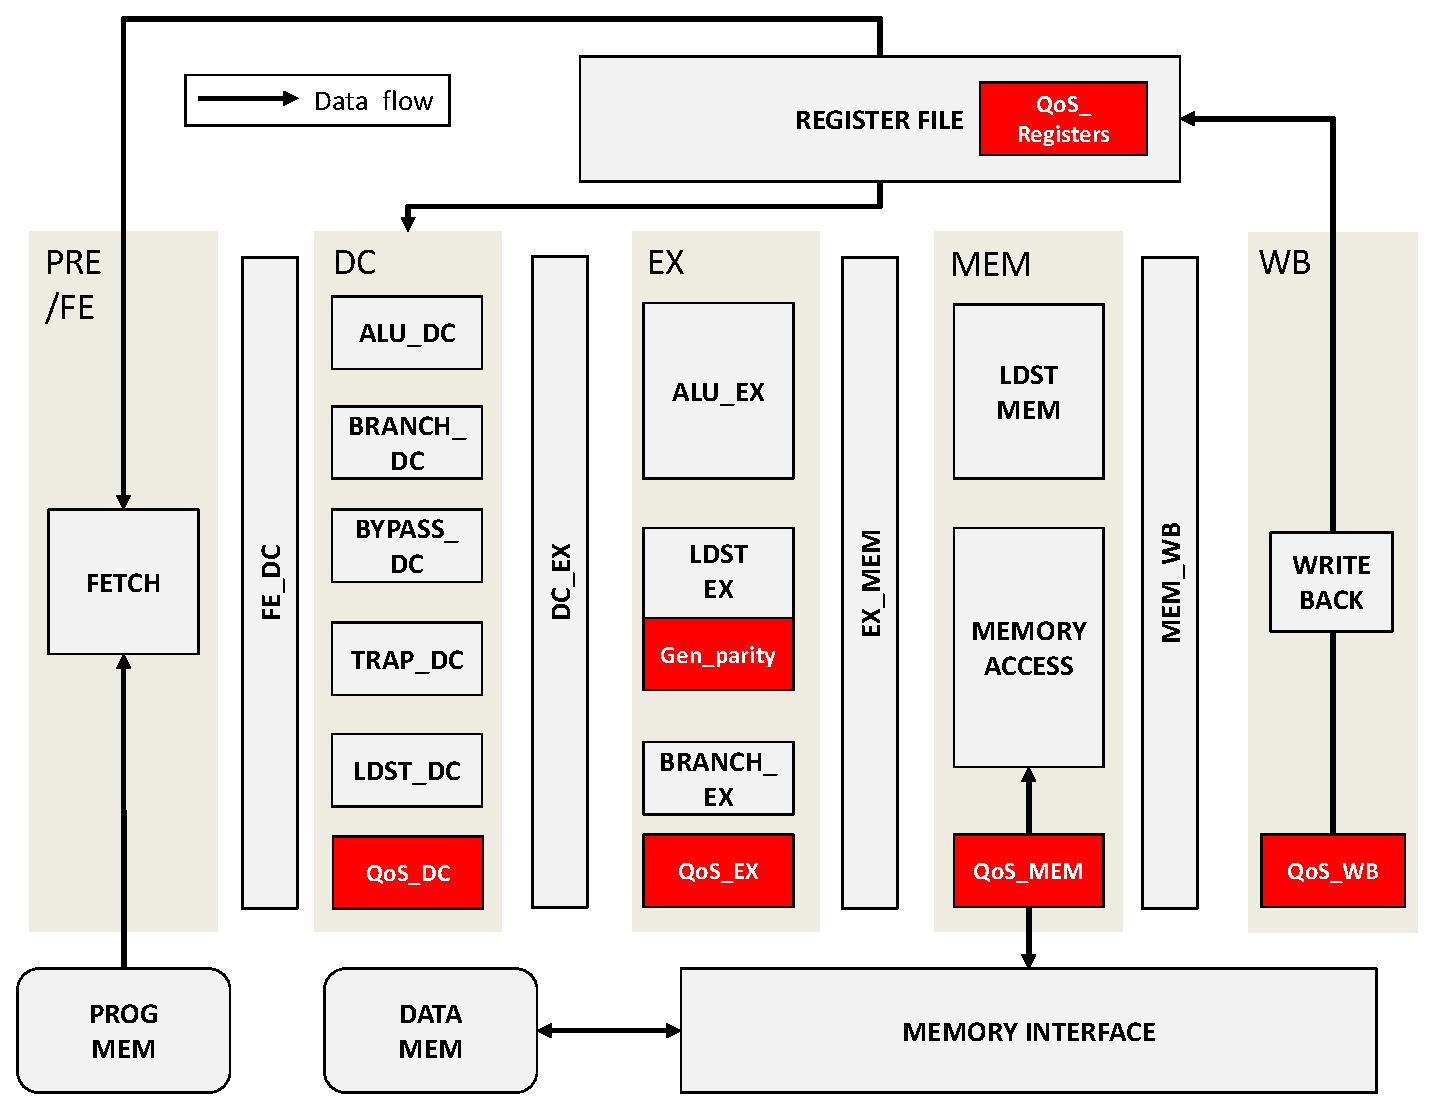
\includegraphics[width=80mm]{./eps/qos_processor}
\caption{Microarchitecture of RISC processor with enhancements for statistical based error confinement}
\vspace{-3mm}
\label{fig:qos_processor}
\end{figure}

\begin{figure}
\centering
\includegraphics[width=90mm]{./eps/qos_arch_explain_date16}
\caption{Introduced modules and their functionality}
\vspace{-3mm}
\label{fig:qos_arch_explain}
\end{figure}
%\vspace{-5mm}

%This has to go in the results
%\begin{figure}
%\centering
%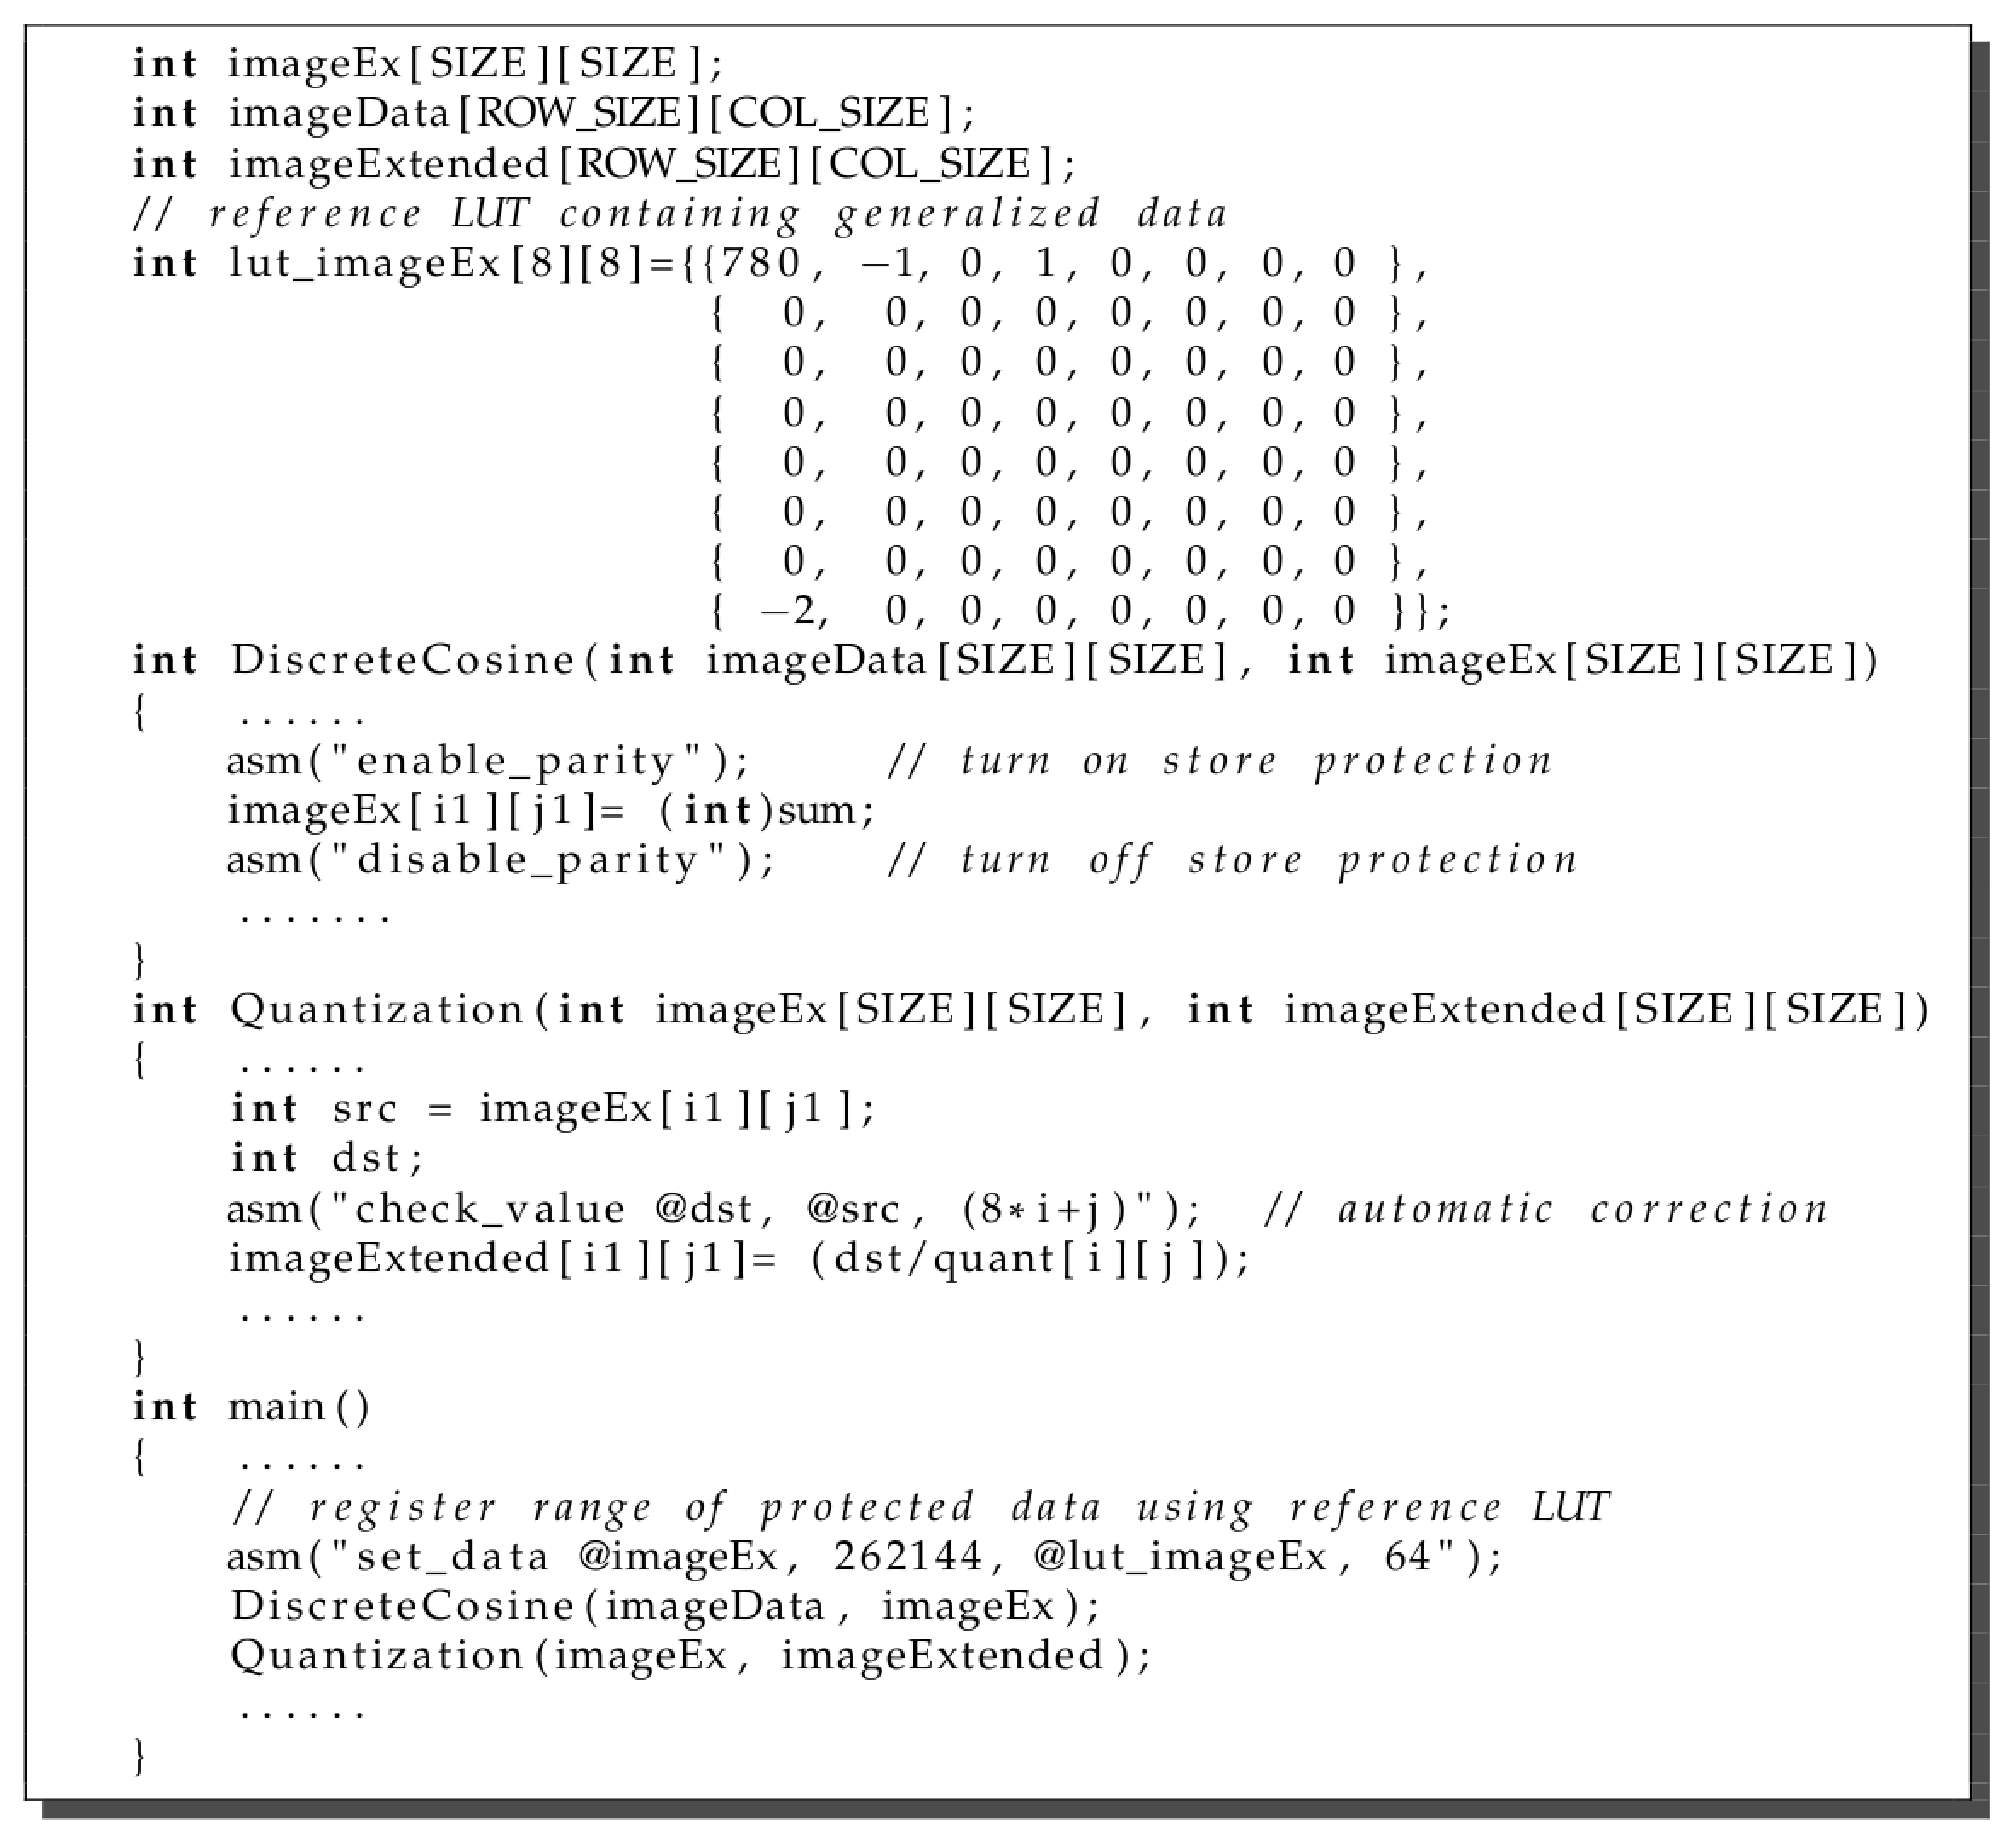
\includegraphics[width=90mm]{./eps/qos_program}
%\caption{Programming example with custom instructions for DCT}
%\label{fig:qos_program}
%\end{figure}

%This has to go in the results
%The architecture is synthesized at 25MHz under 65nm Faraday technology. Table \ref{tab:qos_overhead} presents the synthesis result compared to the original processor. It is observed that the architectural extension incurs huge overheads on the original processor in area and power. Further investigation reviews that the logic and registers which record the memory range of protected data, LUT and parity encoding contribute to such overhead. Additionally, such overhead enables the generic programming environment for similar algorithms, which exhibits the trade-off between hardware usage and programming complexity. However, great saving is resulted from the memory usage as the analysis in Section \ref{sec::soft_overhead}. In terms of critical path, the timing cost only has 4.2\% increment since the longest path of the original design, which goes through the hardware multiplier, remains almost unchanged.

%\begin{table}[hbt]
%\begin{center}
%\caption{Overheads for architecture extension}
%     \label{tab:qos_overhead}
%\begin{tabular}{|c|c|c|c|c|c|}\hline 
%                  & \multicolumn{2}{c|}{\textbf{Area}} & \multicolumn{2}{c|}{\textbf{Power}} & \textbf{Critical} \\ 
%                  & \multicolumn{2}{c|}{\textbf{(NAND equiv.)}} & \multicolumn{2}{c|}{\textbf{($\mu$Watt)}} & \textbf{path} \\ %%\cline{2-5}
%                  & Comb. & Seq. & Dynamic & Leakage & (ns) \\\hline
%Original          & 11789         & 6187       & 206     & 65      & 6.12 \\\hline
%QoS extension     & 26519         & 10663      & 349     & 124     & 6.38 \\\hline
%Increase (\%)     & 124.9         & 72.3       & 69.4    & 90.8    & 4.2  \\\hline
%\end{tabular}
%\end{center}
%\end{table}

%\section{Error Confinement in JPEG Application} \label{sec:jpeg}

JPEG is a commonly used lossy compression technique of digital images, which offers selectable compression degree to trade off between storage size and image quality. JPEG consists of several major steps including color space transformation and down sampling. In this work, we focus on the subsystem shown in Figure \ref{fig:qos_jpeg} which consists of four major blocks, the 2D Discrete Cosine Transformation (2-D DCT), Quantization, De-quantization and 2D Inverse Discrete Cosine Transformation (2-D IDCT). Figure \ref{fig:qos_jpeg} also shows the different stages of the processing image as it propagates through the system. The quality of the output image is evaluated using PSNR \cite{huynh2008scope}. A typical PSNR value for lossy image is 30 dB. The final output image in Figure \ref{fig:qos_jpeg} has a PSNR of 39.22 dB, which is intrinsic tolerable due to the perceptual limitations of human brain.

\paragraph{2-D DCT} is widely adopted in digital image and video processing. It transfers individual $8 \times 8$ image block from spatial domain to frequency domain. The conventional DCT principle could be referred in \cite{gonzalez2009digital} while there exists low power and fault tolerant implementation for 2-D DCT \cite{august2004low}\cite{banerjee2007process}. The output $8 \times 8$ matrix of DCT contains the frequency coefficients which affect the image quality. However, their impacts are non-uniform. According to \cite{banerjee2007process} the first 20 coefficients control 85\% of the input image quality while the rest 44 coefficients have significantly less contribution in improving the image quality. 2-D IDCT is the inverse operation of DCT, which transforms the coefficient in frequency domain back to the spatial domain.

\paragraph{Quantization} is used to compress the image according to different JPEG standard. Each element in the input matrix is divided by a coefficient in the quantization matrix. This usually leads to a matrix with non-zero numbers on the top-left corner while zeros in other part of the matrix. De-quantization is the inverse operation of quantization, which scales up the value by multiply the same coefficient in the quantization matrix.

\begin{figure}
\centering
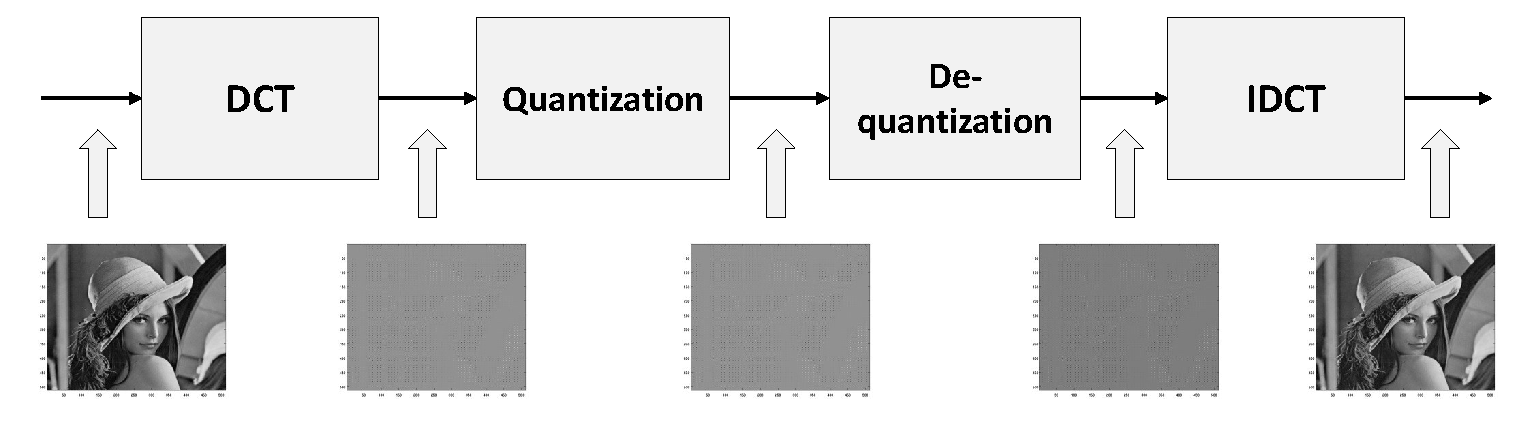
\includegraphics[width=90mm]{./eps/qos_jpeg}
\caption{Subsystem in JPEG application}
\vspace{-3mm}
\label{fig:qos_jpeg}
\end{figure}
%\vspace{-5mm}

The input image which has the resolution of $512 \times 512$ is decomposed into 4,096 matrices of the size $8 \times 8$, where each matrix is being processed individually. Simulation shows that the individual output matrix shares similar pattern, where the top-left corner of both DCT and quantization output matrix exhibits larger number, while the rest ones remains small and even zero for quantization output matrix. Figure \ref{fig:qos_matrix} shows the element wise average matrix for the complete 4,096 individual matrix, which are adopted as the reference matrix for error confinement.

\begin{figure}
\centering
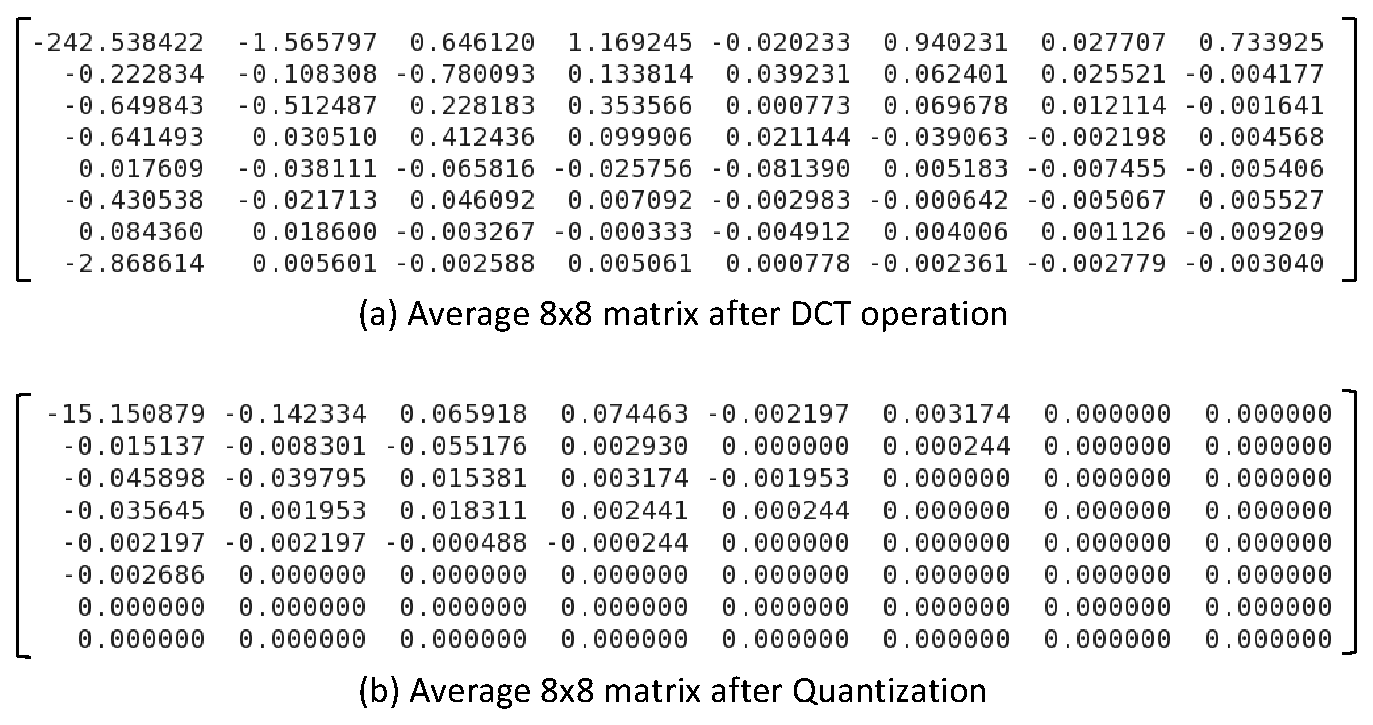
\includegraphics[width=80mm]{./eps/qos_matrix}
\caption{Error confinement matrix for DCT and Quantization Coefficients}
\vspace{-3mm}
\label{fig:qos_matrix}
\end{figure}
%\vspace{-5mm}


\section{Case Study and Statistical Analysis} \label{sec:app}

\subsection{Case Study - JPEG}
To demonstrate the efficacy of the proposed scheme we use as case study the JPEG, which is a widely used    
lossy compression technique of digital images that became a popular application example among error resilient techniques.  
JPEG consists of several stages including color space transformation and down sampling. In this work, we focus on the subsystem shown in Figure \ref{fig:qos_jpeg} which consists of four major procedures. In particular an input image of size $512 \times 512$
is decomposed into 4,096 matrices of the size $8 \times 8$. Then each matrix is being processed individually by the 2D Discrete Cosine Transformation (2-D DCT) \cite{gonzalez2009digital} that essentially  transforms the image into the frequency domain producing the DCT coefficients as output which are then finally being quantized. For the reconstruction of the image De-quantization and 2D Inverse Discrete Cosine Transformation (2-D IDCT) are applied. In general, the quality of the output image compared to the original one is evaluated using the peak signal to noise ration (PSNR) \cite{huynh2008scope} and a typical PSNR value for a lossy image is 30 dB. 

\begin{figure}
\centering
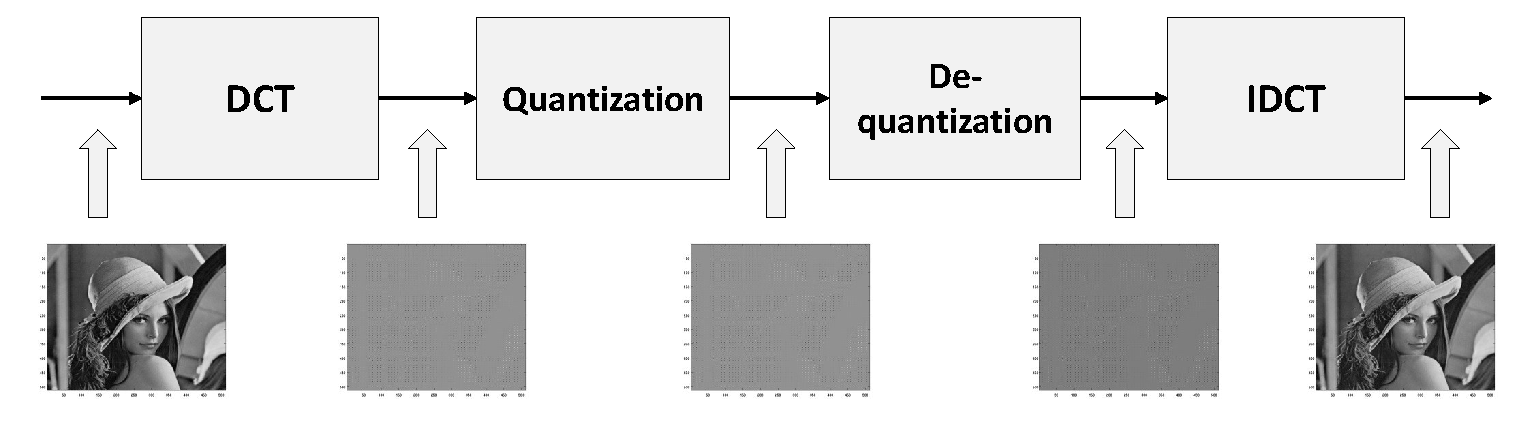
\includegraphics[width=80mm]{./eps/qos_jpeg}
\caption{Subsystem in JPEG application}
\vspace{-4mm}
\label{fig:qos_jpeg}
\end{figure}

\subsection{Statistical Analysis of JPEG}
Following the steps of the proposed approach we statistically analyzed the different stages of JPEG by performing several simulations with different images. Simulations show that the output matrices of DCT and quantization share a similar pattern; the elements at the top-left corner of both DCT and quantization output matrix are larger in magnitude compared to the rest which in most cases are close to zero. Figure \ref{fig:qos_matrix} shows the expected value of each element in the DCT and quantization 
output matrix after averaging their values across 4,096 individual matrices for over 10 images. Such values are used as the reference expected values for replacing the erroneous data in case of a detected memory error in our approach. Note that these values are stored in a LUT that was described in Section III. 

\begin{figure}
\centering
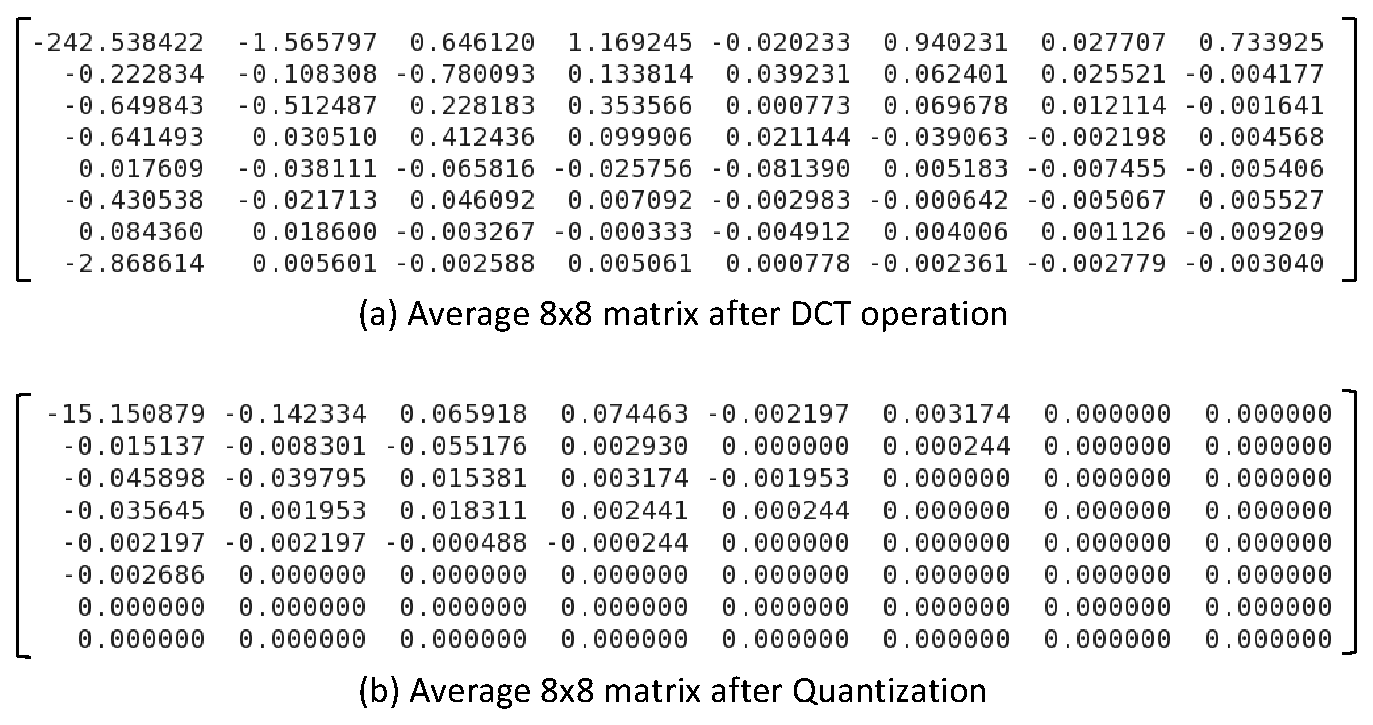
\includegraphics[width=80mm]{./eps/qos_matrix}
\caption{Reference matrix for DCT and Quantization Coefficients}
\vspace{-4mm}
\label{fig:qos_matrix}
\end{figure}


\section{Results} \label{sec:exp}

\subsection{Experimental Setup}
We have modified the RISC processor as discussed in Section II and enabled the injection of bit flips in the memory
locations storing the images and intermediate results of the JPEG. Note that no errors are injected on instruction cache and other registers which are assumed to be adequately protected.     

For detecting errors as we said we encoded each of the 32-bit data of the application with a single parity bit which is sufficient for detecting a single fault. Following the proposed method the new instructions were used as inline assembly to describe JPEG as shown in Figure \ref{fig:qos_program}.  In this example an array containing the reference expected values for the DCT coefficients is defined. 
Within the DCT function, before performing a store to the memory, parity encoding is enabled, which is turned off after a write-store operation. Within the quantization function, the load check is performed whenever a value is read out from the array where the DCT coefficients are stored for replacing it with the relevant expected value in case of an error.

\begin{figure}
\centering
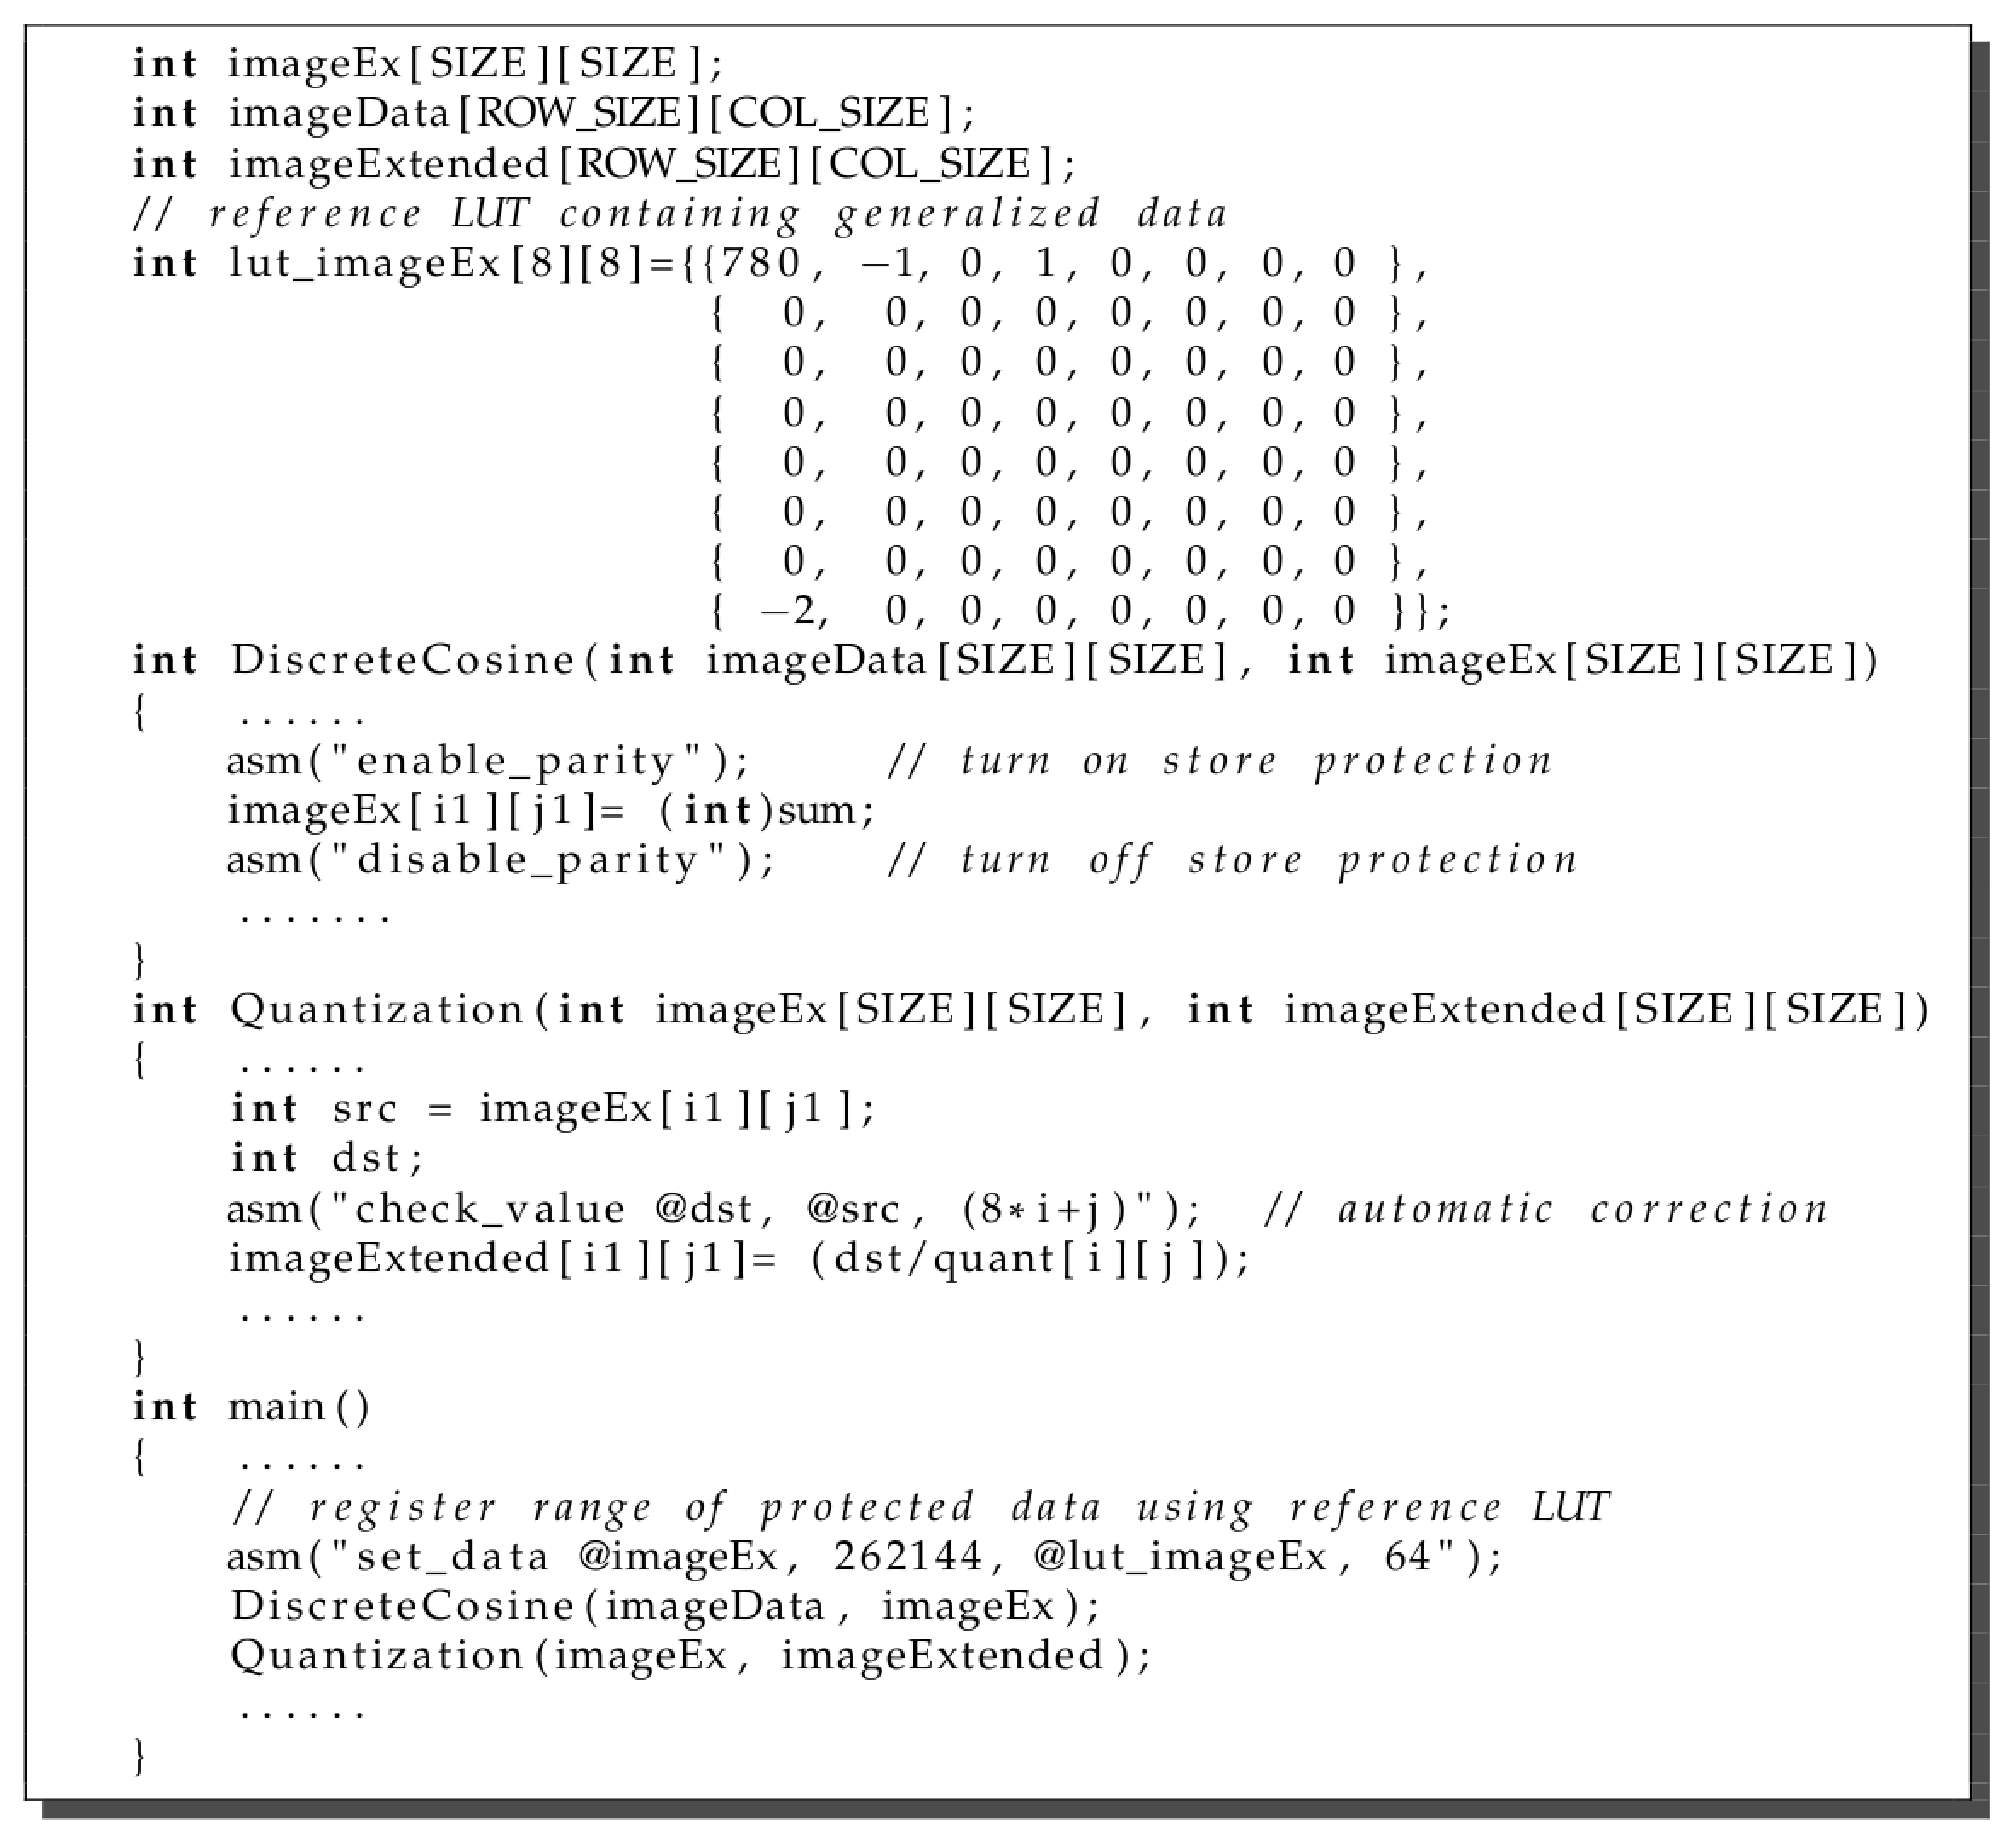
\includegraphics[width=80mm]{./eps/qos_program}
\caption{Programming example with custom instructions for DCT}
\vspace{-4mm}
\label{fig:qos_program}
\end{figure}

The above code was compiled and executed on the modified processor and the performance, power and quality were measured under different error rates as discussed next. Note that for comparison we replicated a similar infrastructure by using a conventional SECDED Hamming code scheme $H[38, 32]$ for the protection of the specific memories (protected by our scheme), which requires 6 parity bits for encoding each 32 bit memory word.  

\subsection{Evaluation of Quality}

Figure \ref{fig:qos_lena} shows the output images and corresponding PSNR values with different numbers of injected bitflips according to typical error rates in 65nm process technology. The results show that in case of 800 and 1000 bitfilps, the output image is degraded by 7.6\% and 41.2\% compared to the error free case.
 
The reason for such a large degradation in case of 1000 bitflips is that two bitflips in the same data word are allowed
which cannot be detected by the single bit parity. Careful examination of our simulations indicated that some of such double bitflips affected words that relate to the first 20 DCT coefficients of the $8 \times 8$ matrix (remember there are 4092 such matrices in each image). As other works have also shown such coefficients control almost 85\% of the overall image quality and thus if the get affected by errors and these are not tackled by any means as in this case then they lead to significant quality degradation. 

\begin{figure}
\centering
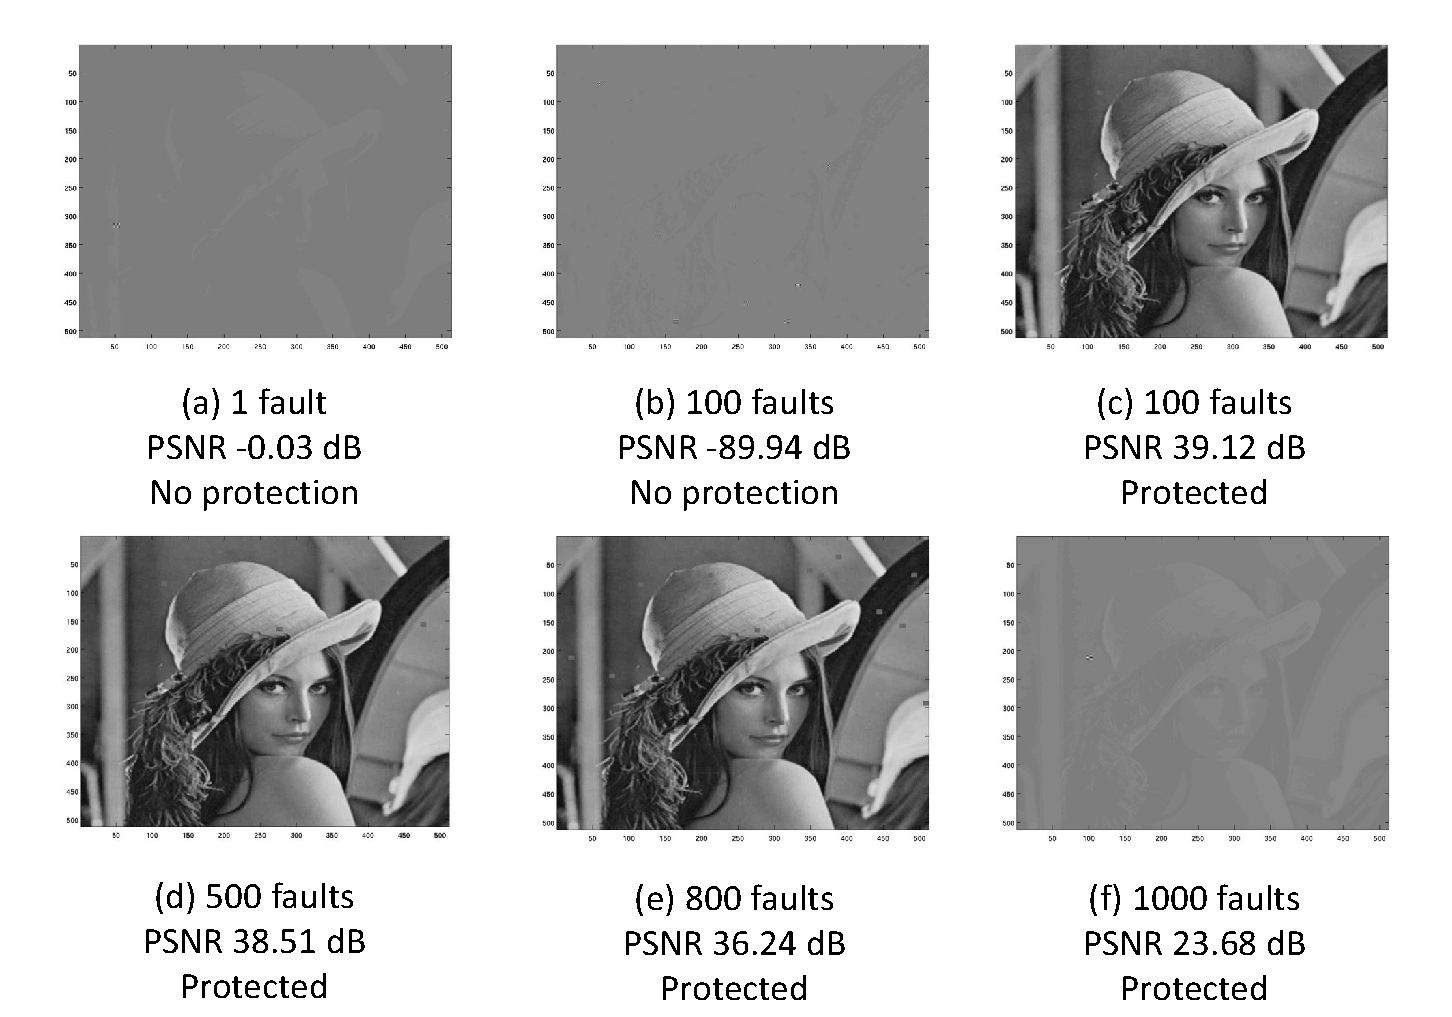
\includegraphics[width=80mm]{./eps/qos_lena}
\caption{Output images under different schemes of error injection}
\vspace{-4mm}
\label{fig:qos_lena}
\end{figure}

As we mentioned we compared the quality achieved by our approach with a SECDED ECC.   
Figure \ref{fig:qos_snr} shows the obtained results in case of protecting the output DCT and quantization coefficients wth the two schemes under different number of single bitflips.  We observed that as the number of the injected single bitflips increases, the output quality (interms of PSNR) achieved by using the proposed approach is slightly less than that achieved by using the ECC scheme. This can be attributed to the fact that in some cases the correct value of the erroneous data that is being substituted by the expected value may indeed lie in the tale of the distribution and thus may be far from the used reference expected value. In these cases the replacement will not be as accurate and thus the quality achieved by our approach may not be as perfect. In any case as we discussed our approach tries to confine the impact of memory errors by essentially approximating erroneous data with their expectation and sometimes such an approximation may not be as good. However, note that the proposed approach still achieves to provide output images with PSNR above 36 dB even under 800 bitflips, closely approximating the error free image.

We observed that above 800 bitflips (when double bitflips are allowed in each word) both methods fail to produce a good enough   image, since neither scheme is able to detect and mitigate from multiple bitflips in single data word. In particular, on one side the SECDED ECC intrinsically cannot correct more than one error in a word and on the other side the single parity bit used to in the proposed scheme cannot detect two bitflips in a word and thus it does not engage the replacement of the erroneous data.

Our results reveal also a different aspect in the JPEG application. In particular, we observed that in case of more than 800 bitflips when double bitflips are taking place in each word then any untreated error in quantization coefficients are far more severe (causing large quality degradation) compared to untreated errors in DCT coefficients. 
This can be attributed to the sparse nature of the quantization coefficients (i.e. most of them are zero) and thefact that any untreated error will significantly alter the expected distribution of these data. 

\begin{figure}
\centering
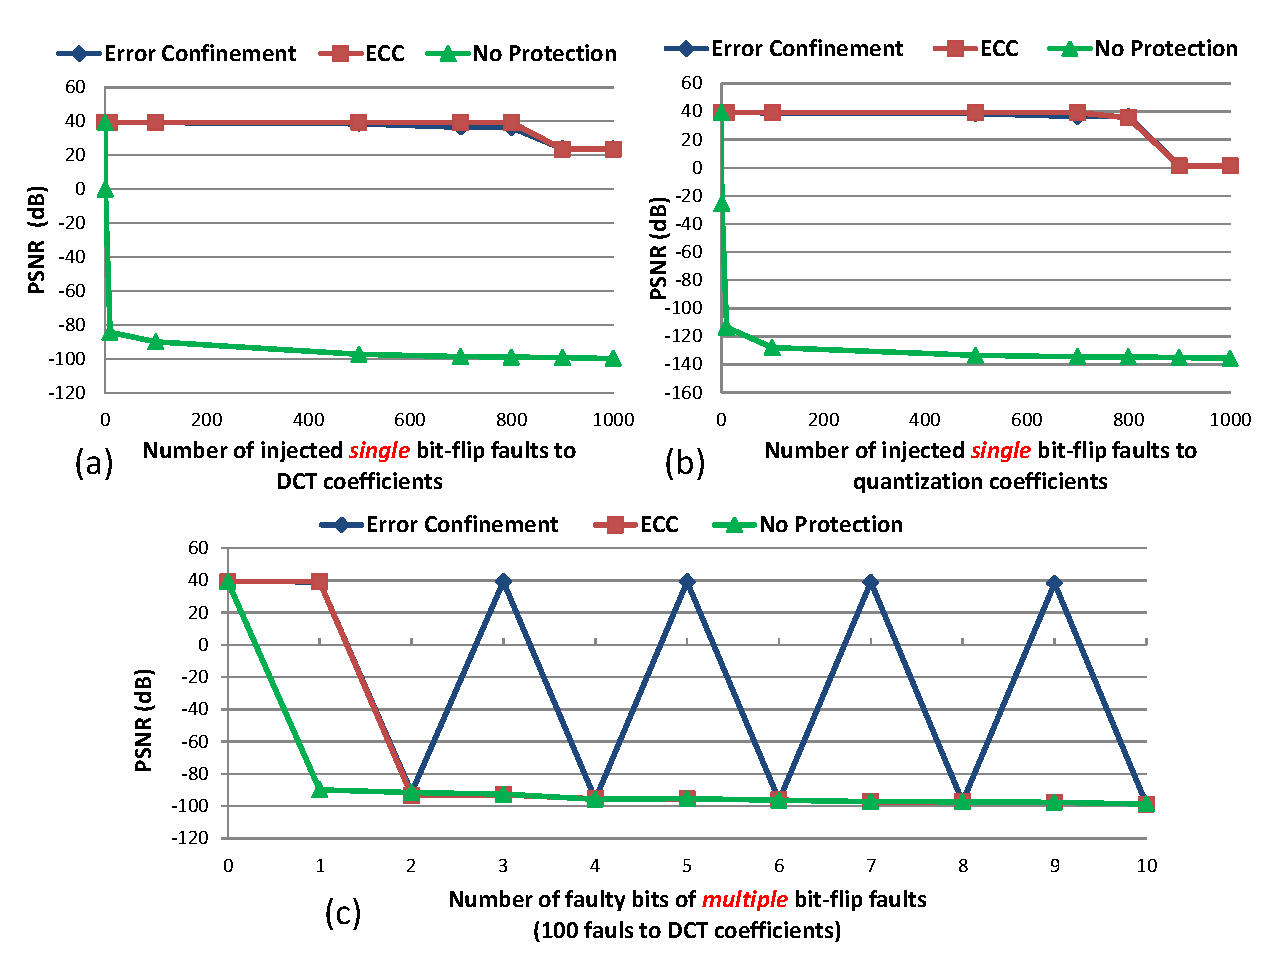
\includegraphics[width=90mm]{./eps/qos_snr}
\caption{PSNR under no protection, proposed scheme and ECC}
\vspace{-4mm}
\label{fig:qos_snr}
\end{figure}

In addition to the above experiments, we have also evaluated the ability of our approach to address multiple bitflips in a single data word by replacing it with the expected reference value. Figure \ref{fig:qos_snr}c) shows the achieved PSNR under different number of bitflips in each word. We can observe that the proposed scheme helps to obtain a PSNR of more than 38dB (for the particular image) in case of odd number of faulty bitcells (when the parity bit can detect the error) while the PSNR degrades a lot in case of even number of faulty bit cells (which cannot be detected by a single parity bit). On the contrary, note that the SECDED ECC even with the use of 6 parity bits fail to address any number of multi bitlfips requiring more complex ECC schemes with much more parity bits. All in all, the proposed approach even with the use of single parity bit is able to address adequately the cases of odd multi flipbits in a single word. The addition of another parity could be employed to improve the capability of error detection which is left for future experimentation. The essential conclusion is that the replacement      
of erroneous data with an expected value suffices to confine the impact of single or even multi memory bitflips.  

\subsection{Performance and Power Results} \label{sec::soft_overhead}
The proposed enhanced processor is synthesized in 65nm Faraday technology and the power, performance and area results
compared to  the original processor are shown in Table \ref{tab:qos_overhead}. Note that the reference processor in this case does not employ any protection scheme and our results in this paragraph try to reveal the overheads involved in enabling 
preferential protection of specific parts of a memory with special instructions as well as the cost of the proposed data replacement scheme.  We can observe that the performance is decreased by only 4.2\% but the instruction extensions for realization of the proposed scheme by a generic programming environment have resulted in large power and area overheads. The extra logic and registers for specifying the protected memory addresses (which is a unique and desirable feature in todays error resilient systems enabled by the proposed extensions), the added LUT and the 1-bit parity encoding are responsible for such overheads. However, note that implementing the same instruction extensions by using 6parity bits as needed by a H(38,32) ECC will result in much larger overheads. 

\begin{table}[hbt]
\begin{center}
\caption{Results for the proposed architecture extensions compared to the reference unprotected processor }
     \label{tab:qos_overhead}
\begin{tabular}{|c|c|c|c|c|c|}\hline 
                  & \multicolumn{2}{c|}{\textbf{Area}} & \multicolumn{2}{c|}{\textbf{Power}} & \textbf{Critical} \\ 
                  & \multicolumn{2}{c|}{\textbf{(NAND equiv.)}} & \multicolumn{2}{c|}{\textbf{($\mu$Watt)}} & \textbf{path} \\ %%\cline{2-5}
                  & Comb. & Seq. & Dynamic & Leakage & (ns) \\\hline
Original          & 11789         & 6187       & 206     & 65      & 6.12 \\\hline
Proposed extensions     & 26519         & 10663      & 349     & 124     & 6.38 \\\hline
Increase (\%)     & 124.9         & 72.3       & 69.4    & 90.8    & 4.2  \\\hline
\end{tabular}
\end{center}
\end{table}

To compare with the SECDED ECC we show the total time required for executing the JPEG application on a processor instance that involves our scheme and on another that implements the ECC. Figure \ref{fig:qos_time_size} depicts the overall execution time of the JPEG application after processing images of different sizes from $8 \times 8$ till $1,024 \times 1,024$ and correcting randomly injected errors (in same locations) with ECC and the proposed scheme.

For small images both methods take similar time since the modules other than the ones shown in Figure \ref{fig:qos_jpeg} dominate the execution time. For images larger than $64 \times 64$ ECC takes significantly longer time compared to proposed scheme. In particular, for an image of size $1,024 \times 1,024$, ECC takes \textbf{3.5}$\times$ more time than the proposed scheme. Note that such overhead will further increase for larger images and more injected errors. 

\begin{figure}
\centering
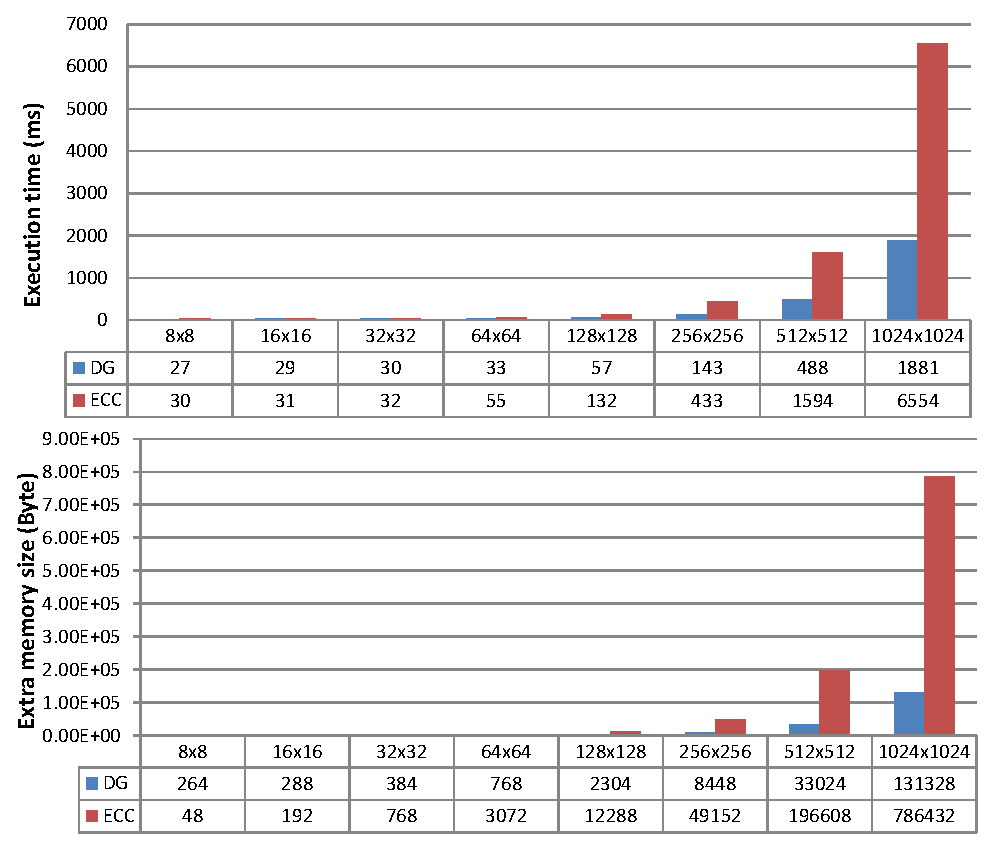
\includegraphics[width=70mm]{./eps/qos_time_size}
\caption{Execution time and data memory usage under Error Confinement and ECC}
\vspace{-4mm}
\label{fig:qos_time_size}
\end{figure}

Although the architecture extension achieves large power overhead, the energy consumption ratio between proposed approach and ECC reduces as image size grows, which is illustrated in Figure \ref{fig:qos_energy}. This is because ECC takes longer time to finish. Starting from image size of $128 \times 128$ the proposed approach consumes less energy than ECC, while the energy benefit increases even further for larger images.

\begin{figure}[hbt]
\centering
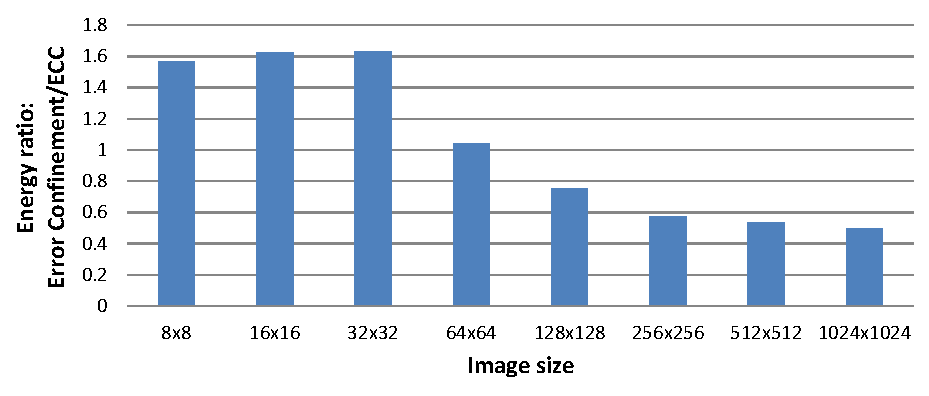
\includegraphics[width=70mm]{./eps/qos_energy}
\caption{Energy ratio between proposed approach and ECC vs image size}
\vspace{-4mm}
\label{fig:qos_energy}
\end{figure}

Another interesting comparison to discuss is the difference in terms of memory usage. As we can also see in Figure \ref{fig:qos_time_size}
the proposed approach uses far less memory compared to SECDED ECC scheme which incurs 18.75\% memory overhead in each protected data word. In particular, for an image of size $1,024 \times 1,024$, ECC requires \textbf{5.99}$\times$ more memory than the proposed error confinement approach.
\section{Conclusion} \label{sec:conclusion}
In this work, a low cost error confinement technique is proposed which exploits the statistical characteristics of target applications and replaces any erroneous data with the best available estimate of that data. The architecture of a RISC processor with custom instructions supporting proposed approach is presented. The benchmarking result shows that the proposed approach achieves far less performance and memory usage overhead than ECC based error detection and correction, while also consumes less energy as image size grows. Further application-level studies using the proposed methodology will be presented in the future.



\scriptsize
%\addtolength{\itemsep}{0 pt}
\renewcommand{\baselinestretch}{0.85}
\bibliographystyle{ieeetr}
\bibliography{./IEEEtranBST/IEEEabrv,relisa}

\end{document}
